\newrefsection
\chapter{B2.a State-of-the-art and objectives}

\eu{(B2.a, B2.b, B2.c: max 15 pages (2 pages for B2.c)}
\eu{Specify the proposal objectives in the context of the state
of the art in the research field. It should be clear how and why the proposed work is important for
the field, and what impact it will have if successful, such as how it may open up new horizons or
opportunities for science, technology or scholarship. Specify any particularly challenging or
unconventional aspects of the proposal, including multi- or inter-disciplinary aspects.}

\TODO{TARGET PAGE COUNT: 3 pages: state of art + vision; 2 pages: methodology overview; 5 pages:
WPs; 3 pages: ethics + risks; 2 pages: resources}

\TODO{as a reference: DECRESIM project: 4 pages on B2.a State of art and
objectives; B2.b ~7 pages on WPs + 2 pages on risk assessment}



\section{State of the art: real-world social robots and impact on the
society}

Social robotics is a disruptive field, with a profound impact on society and
economy~\cite{williams2020social}. A recent report from the United Nations about
the impact of the technological revolution on labour markets stated that AI and
robotics are expected to radically change the labor market world-wide destroying
some job categories and creating others~\cite{bruckner2017frontier}. Social
robotics, however, is still an young, emerging, research-active field. The
expectations are high, in multiple application domains: elderly care, customer
service (in airports and shopping malls, for instance), education, child
development, and autonomous vehicles to name a few~\cite{baillie2019challenges}.
However, whereas both computer-based AI applications, and traditional industrial
robots already have a significant economic impact, social robots have not
reached that point yet. Significantly, the recent failures of several companies
investing in social robotics, like Jibo, Kuri, Willow Garage and Anki, and the
major setbacks of companies like SoftBank, who designed and deployed hundreds of
Pepper robot in their shops, before renouncing a few months later due to the poor
reception by the customers, show that these technologies are not yet
mature~\cite{tulli2019great}.

Indeed, understanding \emph{why} these robots have failed, is one of the
active debate within the Human-Robot Interaction
community~\cite{hoffman2019anki}, with only a handful of qualitative studies on
this question~\cite{dereshev2019longterm,degraaf2017phased}. Proposed
explanations include the lack of perceived usefulness (robot seen purely as a
toy); the limited liveliness of the robot that become rapidly predictable and
repetitive~\cite{lemaignan2014cognitive}; the poor management of expectations,
where user over-ascribe cognitive capabilities that do not match the reality.
The community agrees however that the crux of the issue is achieving long-term
social engagement~\cite{yang2018grand,hoffman2019anki}

Research is however seemingly hitting a wall to further progress towards
socially meaningful long-term interactions. For instance, in their large review
of research in robotics for education, Belpaeme et al.~\cite{belpaeme2018social}
point to the shortcomings that prevent further development of effective,
long-term social robotics in educative settings: the need for a correct
interpretation of the social environment; the difficulty of action selection;
the difficulty of pacing generated behaviours: three issues that underpin
long-term engagement.

Attempts at long-term human-robot interactions are nevertheless becoming more
common~\cite{kunze2018artificial,leite2013social}, with a number of studies
involving social robots deployed in real-world settings (for instance in
schools~\cite{leite2014empathic,westlund2017measuring,
lemaignan2016learning,coninx2016towards}, homes~\cite{degraaf2017phased} and
care centres~\cite{hawes2017strands,winkle2020couch}) over relatively long
periods of time (up to 2 or 3 months at a time). Even though these robots are
typically not fully autonomous, they do exhibit a level of autonomy, either by
handling autonomously a relatively broad range of shallow tasks (eg, a
butler-like robot answering simple questions, like in~\cite{hawes2017strands} or
in the H2020 MuMMer~\cite{heikkila2018where} and FP7
Spencer~\cite{triebel2016spencer} projects), or a narrow, well-specified complex
task (for instance, supporting exercising in a gym, as I did in~\cite{winkle2020couch}).
However, general purpose, long-term interaction is still an open question.


\subsection{Social robotics and vulnerable children}

Application of social robotics to vulnerable children (either hospitalised or
suffering cognitive and/or motor impairments) is an active field of research.
This reflects both the measured efficacy of robot-based intervention, and the
perceived need for additional support for these populations.  Several European
projects have looked at these populations, for instance the FP7 Aliz-e and H2020
DREAM projects: in Aliz-e, \cite{baxter2011long,coninx2016towards} report on how
a social robot can support long-term engagement with diabetic children in
hospital (noting however the rather ``crude'' nature of the created social
interactions, and the limited autonomy of the robot).

A significant body of literature also exist on robotics and autism (see for
instance review by Pennisi et al.~\cite{pennisi2016autism}). This specific
domain has been a fruitful terrain to explore specific aspects of social
cognition in robotics (for instance, related to the Theory of Mind or to the
processing of emotions. See my review in~\cite{lemaignan2015mutual}). This
research draws on the extensive prior research in experimental cognitive
sciences on autism (for instance~\cite{baron1985does, frith1994autism}), and the
focused experimental programme of WP2 will specifically draw from this body of
prior work to evidence the newly developed social modeling capabilities of the
robot.

The experimental programme of \project will take place over two years, first in
Special Education Needs schools (WP5.1), then in a paediatric ward at the
Bristol's Children's Hospital (WP5.2). For both these studies, I will build on
the experience learnt from previous studies in similar environments, with the
novel contributions being both the very long-term interventions (one year each),
and the user-centered methodology that I describe in the following sections.


\subsection{State of art in mobile robotic platforms for social interactions}

Looking specifically at human-sized mobile manipulators with advanced social
features, the choice of robotic platforms is in effect limited.
Table~\ref{robot-comparison} compares the two leading mobile social robots
available on the market today (PAL TiaGo and SoftBank Pepper), along with the
new R1 platform developed by the Italian Institute of Technology (note that the
Fetch Mobile Manipulator has been omitted, as it is functionally similar to
TiaGo).

While not yet on the market, the IIT has offered early access to the platform
for this project.

\begin{table}[h!]
    \caption{Comparison of IIT R1 robot with PAL TiaGo and Softbank Pepper. R1 has been chosen for \project
    for being the only mobile dual manipulator with good navigation and advanced social interaction
    capabilities.}
    \resizebox{\linewidth}{!}{
    \begin{tabular}{@{}p{3cm}p{5cm}p{5cm}p{5cm}@{}}
\toprule
                                           & PAL TiaGo                                                & Softbank Pepper                                                           & \textbf{IIT R1}                                                                                                                              \\ \midrule
\textbf{Social features}                   & Poor (non-expressive head)
        & Expressive, yet fixed, face; limited gaze; approachable & Expressive
        face~\cite{lehmann2016head}; artificial skin for touch-based interactions; approachable \\
\textbf{Perception}                        & Medium (RGB-D camera; laser
        scanner; no microphone)      & Medium (RGB-D; simple mic array; poor
        laser scanner)                      & Good (RGB-D; simple mic array;
        laser scanner)                                                                                                   \\
\textbf{Navigation}                        & Good (however, limited agility due
        to large footprint)   & Poor (weak localisation capabilities)
        & Good (high agility due to Segway-like self-balancing)                                                                                                   \\
\textbf{Safety}                            & Medium (heavy robot; large footprint; non-compliant arm) & Medium (smaller footprint; safe arms; limited stability)                  & Good (smaller footprint; safe arms; dynamic stability)                                                                                       \\
\textbf{Manipulation capabilities}         & Medium (non-anthropomorphic gripper; single arm)         & Limited (poor gripper with low payload; dual arm)                         & Good (anthropomorphic gripper; pressure sensors; dual arm; 1.5kg payload)                                                                    \\
\textbf{Suitability for care environments} & Poor (relatively large, difficult to clear)              & Good (smaller footprint, easy to clean)                                   & Good (smaller footprint, easy to clean)                                                                                                      \\ \bottomrule
\end{tabular}
}
    \label{robot-comparison}
\end{table}



%%%%%%%%%%%%%%%%%%%%%%%%%%%%%%%%%%%%%%%%%%%%%%%%%%%%%%%%%%%%%%%%%%%%%%%%%%%%%%%%%%%%%%%%
%%%%%%%%%%%%%%%%%%%%%%%%%%%%%%%%%%%%%%%%%%%%%%%%%%%%%%%%%%%%%%%%%%%%%%%%%%%%%%%%%%%%%%%%
%%%%%%%%%%%%%%%%%%%%%%%%%%%%%%%%%%%%%%%%%%%%%%%%%%%%%%%%%%%%%%%%%%%%%%%%%%%%%%%%%%%%%%%%
%%%%%%%%%%%%%%%%%%%%%%%%%%%%%%%%%%%%%%%%%%%%%%%%%%%%%%%%%%%%%%%%%%%%%%%%%%%%%%%%%%%%%%%%
\subsection{Methodologies}


The different phases of the \project project build on different methodologies,
from deep machine learning, to qualitative and quantitative field work with
social robots.

\subsection{Construction and characterisation of social embeddings}

The first research objective focuses on the construction and characterisation of
\emph{social embeddings}.

In the context of machine learning, we refer to an \emph{embedding} as a
real-valued vector representation of a typically much higher dimensionality
input. In other words, a representation that encodes high-dimensionality input
(for instance, an image) into a lower-dimensional space. Critically, embeddings
are trained to encode the relationships and semantic nuances that might exist in
the original input space. For instance, two pictures of the same face
transformed with an embedding tuned for facial recognition would yield two
vectors that are similar to each other (i.e., close to each other for a given
metric, usually the cosine distance). As such, the process of embedding not only
condenses high-dimensional information into a more manageable form but also
captures latent associations that might otherwise remain
obscured~\cite{bengio2009learning}.

Unsurprisingly, the training of compact yet semantically-rich embeddings has
been a very active research topic over the last two decades, yielding
exceptional results in machine learning, where the (otherwise high)
dimensionality of real-world percepts might turn common machine learning
tasks like classification or prediction intractable.

While research on embeddings initially focused on data that would intuitively
lend itself well to mathematical transformations (for instance, reducing the
dimensionality of an image, represented as an array of pixel intensities, or
processing sound), it has since then been discovered that many constructs --
physical or not -- can also be \emph{embedded} in a low-dimension numerical
space, while preserving many of their semantics. One of the landmark
achievements in that regard is the work published in 2013 by Mikolov et al. --
themselves building on previous work spanning another decade.  They showed that
embeddings can be computed for \emph{words}, also encoding some of their
semantic meaning~\cite{mikolov2013efficient}, with the famous example of
\emph{embedding(`king') - embedding(`man') + embedding(`woman') $\approx$
embedding(`queen')}. Effectively, a conceptual equivalence of terms, involving
semantics related to gender and social role could be transformed into simple
mathematical additions and subtractions.

This outcome ushered in a decade of intense research on text representation,
ultimately resulting in the current Large Language Models (LLM) like GPT or
Llama2. Most of the recent progress has been enabled by the discovery in 2017 of
the attention-based \emph{Transformers}~\cite{vaswani2017attention} neural
network structure, which brought a boost to the research on natural language
procesing with, for instance, BERT~\cite{devlin2019bert} in 2019 and the family
of GPT models~\cite{wolf2020transformers} in 2020. These large models are
pre-trained on massive text corpora and are typically used for token prediction
(the pre-trained network is fed with a text context, and predicts the next
tokens).

Importantly for this work, these very large pre-trained networks can also be used
to compute text-level embeddings, representing a short text as a numerical
vector~\cite{reimers2019sentencebert,muennighoff2022sgpt}. The resulting
embeddings can be then used to measure text-relatedness for instance, as in the BEIR
benchmark~\cite{thakur2021beir}.

Combining the above concept of text embedding with social situations, \project
will introduce and develop the idea of \emph{social embeddings}. A \emph{social
embedding} is a compact, real-valued numerical representation (a vector) of a
social situation, as experienced by an agent immersed in that social
environment. Following the general idea of embeddings, social embeddings are
designed to encode the \emph{semantics} of the social situation currently
experienced by the agent, facilitating the interpretation of the situation. For
instance, it could make it straightforward to compare two social situation by
simply measuring how similar the two corresponding embeddings are.

The key insight to construct these embeddings is to exploit the social knowledge
already encoded in the latent space of large language models. I will do so by
automatically generating a textual description of the social environment of the
robot (using its existing perception routines), and by transforming this
description into a text embedding via a large language model. By doing so, I
effectively construct an \emph{embedding}, i.e., a projection, of the social
space into a machine-friendly numerical space.


While I have shown in~\cite{lemaignan2024social} that off-the-shelf Large
Language Models can successfully be applied to compute such embeddings, their
expressiveness could be significantly increased by fine-tuning. For instance,
contrastive-learning-based fine-tuning~\cite{hadsell2006dimensionality} has
shown potential for instruction-based text embeddings~\cite{canal2022survey}.
Exploring this and other fine-tuning techniques will be part of the first phase
of the project. Fine-tuning requires appropriately annotated data, whose
acquisition I will also conduct during the project.

Characterising the resulting embedding is largely an open research question. Of
particular interest is the question of the embeddings' latent semantics. For
instance, we can expect that social situations like `two persons chatting
together'; or `a group of three people walking together'; or `one single person
walking towards the robot'; etc. are all semantically distinct, and,
consequently, would belong to distinct regions in the embedding space.
Identifying such clusters to characterize the semantic topology of the embedding
space would enable not only to measure how similar two social situations are,
but also characterize key features of the current situations.  This idea is
related to e.g. the recent investigation by Sun and
Nelson~\cite{sun2023topological} on latent semantics of sentence embeddings.


\subsubsection{Applications of Social Embeddings}


\paragraph{Real-world social situations}

by clustering a diverse set of social situation embeddings, it should
be possible to isolate key prototypical social situations, to which
rules, norms, behaviours could be associated. A robot could then 
recognise when it encounter such situations, and also
estimate the \emph{dynamics} of the current situation, i.e. towards what
other situation it is headed;

In addition to data science techniques, fieldwork

I have an extensive experience in running field studies with social robots~\cite{hood2015when, lemaignan2016learning, jacq2016building,
        baxter2015wider,kennedy2016cautious,senft2018robots}, at home~\cite{mondada2015ranger}

\paragraph{Generative Adversarial Network}

as vector representations, social encodings lend themselves well to
        many downstream machine learning tasks, for instance socially-appropriate behaviour
        generation, or situated interactive machine learning

\project aims at significantly advancing the state of the art in this regard, by
combining two recent techniques: (1) generative neural networks for affective
robot motion generation~\cite{marmpena2019generating,suguitan2020moveae} (with
training data created with an expert choreographer); (2) interactive machine
learning in high-dimensional input/output spaces, where I have shown with my
students promising results for generating complex social
behaviours~\cite{senft2019teaching, winkle2020couch} that fully involve the
end-users~\cite{winkle2018social}. Modulating (1) with the learnt features of
(2), I target a breakthrough in robots' social behaviours generation: the
generation of non-repetitive, socially congruent and transparent social
behaviours (including gestures but also gazing behaviours and facial
expressions).


\paragraph{Interactive machine learning}

contextualised lifelong adaptation of the robot's
behaviours, by augmenting existing interactive machine
learning techniques (`user in-the-loop' learning) with
representations of the social environment;


\subsubsection{Responsible Robotics}

Actual utility and long-term acceptance requires genuine involvement of the
end-users at every step of the design process. This is at odds with the common,
engineering-centered practise of first developing robots and algorithms \emph{ex-vivo}, in
lab, and then placing a (semi) final product in the hands of the users, hoping
for adoption. Adoption, however, is the result of a long process of \emph{mutual
modelling}~\autocite{sabanovic2010robots}, where
the social role of the robot is slowly constructed from its real world, in-context
usage.

This foundational insight requires the conceptual framing and development of new
research methodologies.  I have started to explore these questions in some of my
previous work~\autocite{senft2016sparc,winkle2019effective,winkle2021leador},
and my research program aims at significantly developing this line of research
to tackle more complex, long-term application domains.

One of the major challenge arising with more complex application domains is
however the combinatorial growth of the problem space. Indeed, none of the
current control paradigms or cognitive modelling techniques are able to
successfully predict context- and task-appropriate sequences of behaviours
for socially-useful autonomous robots.

\vspace{0.4em}

My research programme aims at tackling this challenge with two key insights: (1) the
representation complexity of the social and spatial environment of the robot 
can be dramatically reduced by treating it as an \emph{embedding} problem and
applying modern machine learning techniques (like GANs) to design and compute
\emph{social embeddings}; (2)
modern transformers and attention-based~\autocite{vaswani2017attention} machine learning
architectures have demonstrated long-term modelling
capabilities on complex language domains~\autocite{ouyang2022training} that could
in principle be equally applied to action sequence generation for
robots. Initial explorations of this second insight have started to
emerge~\autocite{brohan2022rt,vemprala2023chatgpt}, but none of these early research
efforts consider the complexity of human interactions.

\vspace{0.4em}

My research program will research how these insights can be effectively
operationalized, with a scientifically ambitious
and highly technical work program. It includes basic research and conceptual
framing; extensive, beyond-state-of-art, technical developments; and an
ambitious experimental program, centered on long-term `user in-the-loop' data
collection via field deployments of social
robots in public spaces -- and primarily in the healthcare and elderly care
environment.

%%%%%%%%%%%%%%%%%%%%%%%%%%%%%%%%%%%%%%%%%%%%%%%%%%%%%%%%%%%%%%%%%%%%%%%%%%%%%%%%%%%%%%%%
%%%%%%%%%%%%%%%%%%%%%%%%%%%%%%%%%%%%%%%%%%%%%%%%%%%%%%%%%%%%%%%%%%%%%%%%%%%%%%%%%%%%%%%%
%%%%%%%%%%%%%%%%%%%%%%%%%%%%%%%%%%%%%%%%%%%%%%%%%%%%%%%%%%%%%%%%%%%%%%%%%%%%%%%%%%%%%%%%
%%%%%%%%%%%%%%%%%%%%%%%%%%%%%%%%%%%%%%%%%%%%%%%%%%%%%%%%%%%%%%%%%%%%%%%%%%%%%%%%%%%%%%%%

\section{\project aim and objectives: Responsible robots for long-term social engagement}

%\begin{figure}
%    \centering
%    
\includegraphics[width=0.9\linewidth]{figs/wizme+dolls}
%    \caption{Early prototyping for the \project project: a pet-like robot that could
%    mediate child-child interactions, and support group activities like active story-telling.}
%    \label{early-prototype}
%\end{figure}



%
%\begin{figure}
%\centering
%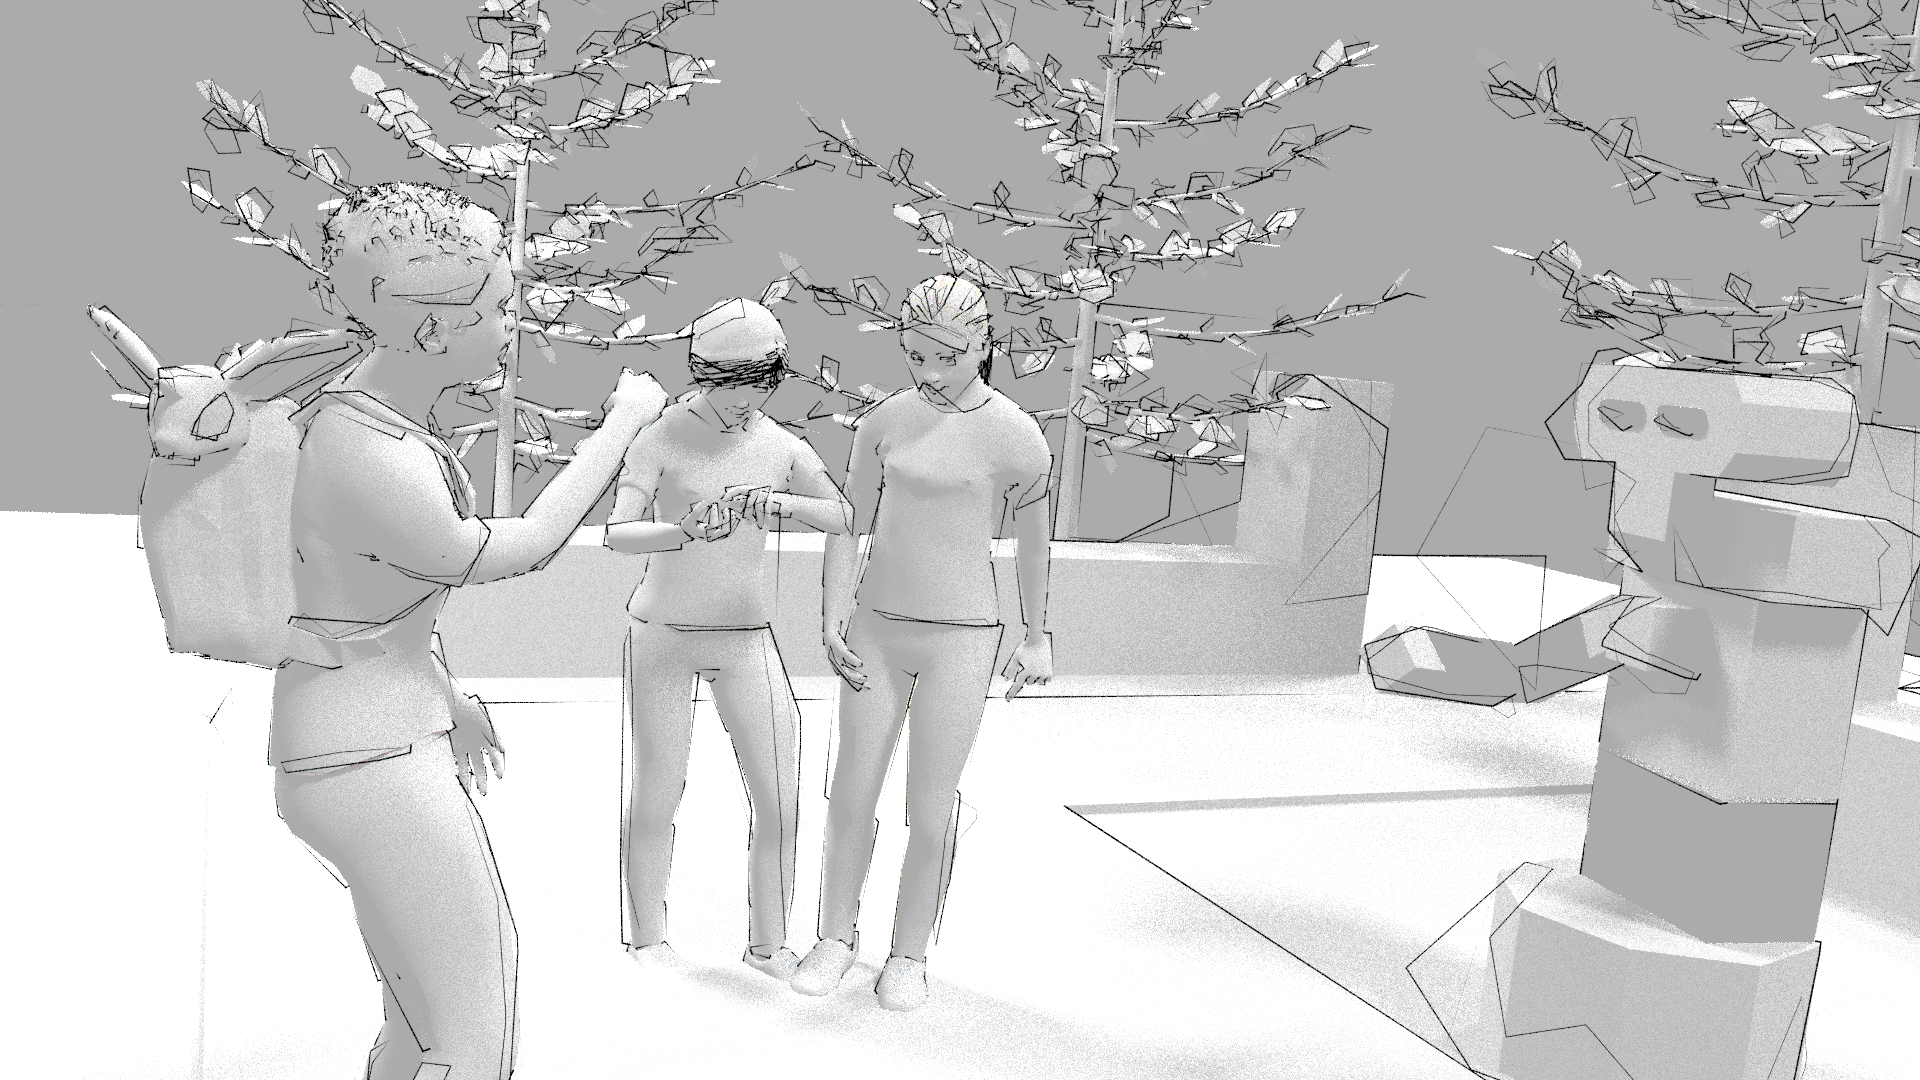
\includegraphics[width=0.9\linewidth]{figs/rHHI-1}
%\caption{A child, just arriving in a new school, tries to integrate with other
%    children -- in such a situation, should the robot decide to help to break the ice? What
%    are the socio-cognitive peceptual and behavioural capabilities required to
%    make that decision?}
%\label{fig:rHHI}
%\end{figure}
%

The overall aim of the \project project is to \textbf{create, sustain and better
understand the dynamics of responsible long-term social human-robot
interactions}.

This broad aim translates in three key research questions that we seek to
address over the course of the project:

\paragraph{\bf RQ1:} what are the public expectations with respect to the role of social
        robots? Can we collectively design principles ensuring safe, beneficial, socially
        acceptable robots? 

\paragraph{\bf RQ2:} what AI is required to sustain long-term engagement between end-users
        and a robot? In particular, how to provide a robot with an understanding
        of its own social environment? How to create behaviours that are not
        repetitive or overly predictable?

\paragraph{\bf RQ3:} what new ethical questions are raised by long-term social interaction
        with an artificial agent? In particular, how to balance autonomy of the
        robot with behaviour transparency and human oversight?

\vspace{0.5em}
\noindent The \project objectives are built around these three questions.

\paragraph{\bf O1: conceptual framing} I will investigate the basic principles
of responsible social interactions, that must form the foundations of a socially
useful robot, accepted and used in the long run. I will answer questions like:
What should motivate the robot to step in and attempt to help? What social norms
are applicable to the robot behaviours? Using user-centred design and
participatory design methodologies, I will identify the determinants and
parameters of a responsible social intervention, performed by a socially-driven
robot, and formalise them in guidelines. This objective aims at addressing RQ1,
and is realised in WP1.

\paragraph{\bf O2: real-time social modeling} I will significantly extend and integrate
the current state-of-art in spatio-temporal modeling (so-called \emph{situation
assessment}) with recent research in social state modeling, to create the novel
cognitive capability of artificial \emph{social situation assessment}, enabling
the robot to represent in real-time the social dynamics of its environment. This
objective addresses one part of RQ2, and is investigated in WP2.


\paragraph{\bf O3: congruent social behaviours production} Using the
state-of-the-art in generative neural networks, combined with data acquired from
an expert choreographer, I will create a novel way of producing non-repetitive,
socially-congruent, expressive motions. This will be integrated with novel
\emph{sound landscapes} to create a beyond-state-of-art, non-verbal yet highly
expressive,  action and communication system for the robot. This objective
addresses another part of RQ2, and is the focus of WP3.

\paragraph{\bf O4: embodied AI breakthrough} I will integrate long-term social
goals, arising from the interaction principles of \textbf{O1}, with the social
modeling capability of \textbf{O2} and the behaviours production of \textbf{O3}
into a principled, goal-driven cognitive architecture. The breakthrough will
come from combining these long-term social goals with bottom-up action policies,
designed and learnt from the end-users using human-in-the-loop reinforcement learning.
This will result in robot behaviours that are perceived as purposeful and
intentional (long-term goals), while being shaped by a
user-created and user-controlled action policy.

I will specifically test \ul{two hypotheses}: first, I hypothesise that long-term
social goals, if suitably co-designed with the public and stakeholders, and
properly integrated into the robot as a \emph{social teleology}, will create the
perception that the robot is intentional and purposeful. This will in turn
elicit sustained engagement from its human users.

Second, I hypothesise that human-in-the-loop machine learning can be used to
ensure an additional layer of human oversight and a level of behavioural
transparency.  Human-in-the-loop reinforcement learning -- as implemented in the SPARC
approach that I have developed and already used in complex social
environments~\cite{senft2017supervised, senft2019teaching, winkle2020couch} -- relies
on a end-user `teacher', initially fully controlling the robot (teleoperation)
while it learns the action policy, and then progressively relinquishing control
up to a point where the robot is effectively autonomous. As argued
in~\cite{senft2019teaching}, this approach leads to increased control and
ownership of the system, and as a result, increased trust.

This addresses RQ2 and RQ3; however it also raise an additional question: how to
arbitrate between a top-down action policy arising from the long-term goals, and
the bottom-up action policy learnt from the end-users? This question leads to
objective {\bf O4'}: The design of a policy arbitration mechanism that preserve
the robot's long-term intentional behaviour, while effectively guaranteeing human
control, ownership and oversight. {\bf O4} and {\bf O4'} are addressed in WP4.

\paragraph{\bf O5: ambitious field research} Finally, the last objective of the
\project project is to demonstrate the effectiveness of my approach in complex,
real world conditions. This means deploying the \project robots into existing
social eco-systems that are sufficiently complex, yet open to explore novel
social interactions. My objective is also to show that this real world
deployment can be successfully driven by `end-to-end' involvement of all the
end-users and stakeholders: from defining the robot role, from the different
perspective of each of the end-users, to actually designing and `teaching' the
robot what to do. This is the focus of WP5.


\begin{framed}

\noindent\bf Together, these five objectives build a coherent and realistic pathway towards
addressing the overall aim of \project: creating, sustaining and better
understanding the dynamics of responsible long-term social human-robot
interactions.

\end{framed}

%%%%%%%%%%%%%%%%%%%%%%%%%%%%%%%%%%%%%%%%%%%%%%%%%%%%%%%%%%%%%%%%%%%%%%%%%%%%%%%
%\subsection{The case for robot-supported human-human interactions}
%
%This change of paradigm (rHHI) will have far reaching impact on the place that
%we collectively assign to social robots in the society; it will help to
%structure the public debate by providing the framework to look at human-robot
%interactions in term of their net social utility.  As such, \textbf{the first
%outcome of \project will be researching, defining and implementing the
%conceptual framework that we need to ensure trustworthy and socially responsible
%robots in our societies}.
%
%Indeed, in a time where robots are on the verge of becoming pervasive in our
%daily human environment, can we ensure 'by design' that robots are to become
%powerful tools to support more and better, positive interactions \emph{between
%the people themselves}, and build a stronger, more cohesive society? Beyond
%Human-Computer Interaction (HCI) and Human-Robot Interaction (HRI), \project is
%a forward-looking, ground-breaking project that aims at establishing
%\textbf{Robot-supported Human-Human Interactions (r-HHI)} as the next step
%toward a Responsible AI: \textbf{the scientific investigation of how social
%robots can create, shape and support strong, sustained, positive
%\emph{human-human} relationships}.
%
%As a researcher who has been working for the last 12 years in the field of
%human-robot interaction (and child-robot interaction in particular), I have been
%a direct witness -- by being one of the architects -- of the crossing of a
%critical milestone: the emergence of \textbf{long-term social interactions}
%between robots and humans. Over the last two years in particular, we observe an
%explosion of the number of studies involving social robots, deployed in
%real-world settings (schools, care centres) over relatively long periods of time
%(up to 2 or 3 months at a time)~\cite{kunze2018artificial,leite2013social}. Even
%though these robots are rarely fully autonomous, they do already show high
%levels of autonomy~\cite{senft2019teaching}, with full autonomy in
%sight~\cite{hawes2017strands}.
%
%Due to the complex interplay between the socio-psychological determinants of the
%interactions, the technical implementation, and the multiple ethical mechanisms
%that have to be built-in the system, it is difficult to build one coherent and
%consistent perspective on the whole question. Indeed, the conceptual,
%intellectual framework emcompassing both the internal cognitive mechanisms
%required by socially intelligent robots, as well as their role and impact in the
%society, only exists in fragmented, disconnected pieces~\cite{citeneeded}.
%
%
%The lack of such a proper conceptual framing is a critical issue: for robots to
%have a positive impact on the society, with strict ethical and privacy-related
%safeguarding, it is urgent that the wider academic and intellectual communities,
%beyond technologists, embrace this question and build up the debate on the
%acceptability of robots in our society. And \textbf{this also calls for a major
%re-thinking of the traditional paradigm of Human-Robot Interaction}.
%Tradionally, individual cognitive functions (like natural language processing,
%emotion recognition, proxemics-aware navigation) are implemented in robots, with
%the ill-supported assumption that 'the more available functions, the more
%socially-capable the robot'. This assumption is questionable, and, at any rate,
%does not address the 'why': why does the robot decides to do what it does? What
%drives the behaviour of the robot? The case for \emph{teleological} (ie
%goal-driven) robotic architectures has been made in the
%past~\cite{wrede2012towards}, but only effectively realised for relatively
%simple cognitive systems (like curiosity-driven robot
%animals~\cite{oudeyer2005playground} or motor babbling in infant-like
%robots~\cite{forestier2017unified}). However, socially-driven robots,
%participating in complex interactions with humans, have been barely
%investigated. We need to create a new social purpose, a new social teleology to
%drive the development of social robots.  Indeed, \textbf{being socially-driven
%to do 'good' is essential in ensuring trustworthy, socially responsible robots}.
%Nutrured by decades of research in understanding human social cognition and its
%social motivations, one of the key purpose of \project is to \textbf{research
%and build a principled and socially-driven cognitive architecture} for
%tomorrow's social robots. This socially-driven, teleological architecture,
%intrinsically designed to \textbf{support stronger, positive human-human
%interactions} is what underpins the concept of \emph{robot-supported human-human
%interactions}.

%\subsection{Key scientific challenges and research questions}
%
%Socially intelligent robots require unique, beyond state-of-the-art,
%capabilities to \emph{(1)} understand the social interactions (social
%situation awareness), \emph{(2)} autonomously decide the best course of action for
%short-term and longer-term social influence, and \emph{(3)} perform the
%appropriate social actions and exert said influence in an appropriate,
%responsible manner.
%Not only the required technology is itself beyond state-of-the-art (and will be
%researched and integrated in WP2, WP4 and WP3), but the
%interplay between technology, socio-cognitive psychology, privacy and ethics is
%only starting to be researched and understood. \project offers an
%strong vision and an ambitious, evidenced-based, methodology to significantly
%advance our understanding of this multi-faceted problem.
%
%Over the course of 5 years, I will investigate hypotheses H1 and H2
%by addressing the following research questions:
%
%\begin{itemize}
%    \item \textbf{R1} [conceptual framing]: what are the basic principles of
%        responsible social interactions, that must form the foundations of a
%        socially useful robot, accepted and used in the long run? What should
%        motivate the robot to step in and attempt to help? What are the
%        determinants and parameters of a social intervention, performed by a
%        socially-driven robot, to support positive human-human social
%        interactions? How to balance social utility and social responsibility?
%
%    \item \textbf{R2} [implementation level]: how will these principles
%        be integrated into a principled, socially-driven teleological
%        architecture for autonomous robots? How this should be combined with
%        bottom-up action policies, designed and learnt from the end-users? How
%        can we ensure `by design' that the resulting AI will generate useful yet
%        responsible, trustworthy, human-centered robot behaviour?
%
%    \item \textbf{R3} [technology level]: where are the technological gaps in
%        artificial social modeling and cognition, that prevent the actual
%        realisation of a robot capable of effective social support, sustained
%        over long period of time? How can we fill them?
%
%    \item \textbf{R4} [experimental level]: can we demonstrate in complex, real
%        world conditions, the effectiveness and usefulness of the
%        robot-supported human-human interaction paradigm? Can we do so by
%        involving the end-users at every stage of the design, implementation and
%        testing cycle?
%
%\end{itemize}
%
%
%
%\project is also a highly technical project, who aims at significantly
%pushing the state-of-the-art in autonomous social robotics. Indeed, in \project, we will
%\textbf{implement the AI required for robots to effectively support
%human social interactions}.  In that sense, this research is also
%ground-breaking in regards to its technical objectives. In \project, robots will
%be able to understand complex social dynamics, and generate appropriate social
%responses, in a fully autonomous way.  Extending the current line of research of
%the PI, we will identify, implement, and integrate the a broad range of cognitive functions into a
%principled, socially-driven, and trustworthy socio-cognitive architecture for
%robots. This is the second major expected scientific outcome of \project.

%%%%%%%%%%%%%%%%%%%%%%%%%%%%%%%%%%%%%%%%%%%%%%%%%%%%%%%%%%%%%%%%%%%%%%%%%%%
%%%%%%%%%%%%%%%%%%%%%%%%%%%%%%%%%%%%%%%%%%%%%%%%%%%%%%%%%%%%%%%%%%%%%%%%%%%
%%%%%%%%%%%%%%%%%%%%%%%%%%%%%%%%%%%%%%%%%%%%%%%%%%%%%%%%%%%%%%%%%%%%%%%%%%%
\section{Interdisciplinary nature of the research programme}

\project paves the way for a better understanding of the societal challenges
raised by the rapid development of AI and robotics. Grounded in both the
psycho-social literature of human cognition, and the latest technological
advances in artificial cognition and human-robot interaction, the project
delivers major conceptual, technical and experimental contributions across
several fields: AI, ethics, sociology of technology, intelligent robotics,
learning technology. As such, \textbf{\project builds bridges across
multiple disciplinary boundaries}.

\project delivers this programme by building on a range of multidisciplinary
methods, including user-centered design; ethnographic and sociological
investigation; expressive non-verbal communication, including dance and
puppetering; embodied cognition; symbolic AI; neural
nets and sub-symbolic AI; interactive machine learning.

Accordingly, the project builds on a \textbf{strong interdisciplinary team}: the
post-docs directly recruited on \project will have backgrounds in sociology of
technology (PD1), cognitive modeling (PD2), machine learning (PD3), cognitive
robotics (PD4). Additional expertise will be recruited to provide specific
support: the \project Ethics Advisory Board will contribute expertise to guide
the work on ethics; Dr. Newbutt will provide expertise in learning technologies
and cognitive impairment; Dr. Meckin will provide expertise in sound-based
expressive communication; the WeTheCurious science centre will provide training in
large-scale public engagement; the Bristol Children's hospital will bring the
required expertise in working with young patients; the RustySquid company will provide expertise in
expressive arts and puppetering.

%%%%%%%%%%%%%%%%%%%%%%%%%%%%%%%%%%%%%%%%%%%%%%%%%%%%%%%%%%%%%%%%%%%%%%%%%%%
%%%%%%%%%%%%%%%%%%%%%%%%%%%%%%%%%%%%%%%%%%%%%%%%%%%%%%%%%%%%%%%%%%%%%%%%%%%
%%%%%%%%%%%%%%%%%%%%%%%%%%%%%%%%%%%%%%%%%%%%%%%%%%%%%%%%%%%%%%%%%%%%%%%%%%%
%\section{Impact of the \project project}
%\TODO{THIS SECTION IS STILL WORK-IN-PROGRESS}
%
%Academically, the \project project represents a timely combination of
%very recent advances in supervised machine learning for social robot
%behaviour with a creative and interdisciplinary approach to the design
%and automation of social robot behaviour. 
%We will publish \project results in interdisciplinary and high-profile
%discipline-specific journals (eg. Science Robotics; Frontiers in AI and
%Robotics; Transaction in Human-Robot Interaction) and conferences (eg. AAAI,
%HRI, RSS).
%
%The dataset of social behaviours and social signals we will create and
%distribute represents a one-in-a-kind resource for the human robot
%interaction community, and the human data collection will be
%transferable to research in other domains such as human-computer
%interaction.
%
%As \project will be deployed in a living lab environment, there is
%significant scope for public outreach/engagement and media coverage,
%which we will work with the BRL's media manager to maximise.
%
%
%\project aims at building unique European capacity to assert leadership in this
%domain, and, beyond the specific deliverables of this 5-years project,
%establishing the PI as a world-leader in goal-driven, socially-responsible
%robotics.


%%%%%%%%%%%%%%%%%%%%%%%%%%%%%%%%%%%%%%%%%%%%%%%%%%%%%%%%%%%%%%%%%%%%%%%%%%%
%%%%%%%%%%%%%%%%%%%%%%%%%%%%%%%%%%%%%%%%%%%%%%%%%%%%%%%%%%%%%%%%%%%%%%%%%%%
%%%%%%%%%%%%%%%%%%%%%%%%%%%%%%%%%%%%%%%%%%%%%%%%%%%%%%%%%%%%%%%%%%%%%%%%%%%
\newpage

{\let\clearpage\relax\chapter{B2.b Methodology}\label{research-methodology}} % prevent page break before chapter

\TODO{context setting: cf work on image retrieval in SPRING (WP2) -> able to
describe 'where we are' from 3D map, describing environment with tools like
LLaVa/MiniGPT4}

\TODO{get stuff from ElderlyDo projects (eg, data collection)}


\eu{Describe the proposed methodology in detail including any key intermediate
goals. Explain and justify the methodology in relation to the state of the art,
and particularly novel or unconventional aspects addressing the
'high-risk/high-gain' balance. Highlight any intermediate stages where results
may require adjustments to the project planning. In case you ask that team
members are engaged by another host institution their participation has to be
fully justified by the scientific added value they bring to the project.}


\section{Workpackages overview and interrelations}\label{workpackage-interrelations}


The four research questions previously listed are addressed across five
work-packages: \textbf{WP1} is dedicated to the conceptual framing of the
project (R1) and the identification of interaction principles; \textbf{WP2}
extracts from these principles the set of requirements in term of
socio-cognitive capabilities for the robot (R3), and implement them; in parallel
to WP2,  \textbf{WP3} looks at how social robots can generate congruent social
behaviours (R3); \textbf{WP4} transposes the conceptual framework of WP1 into a
principled cognitive architecture and integrates together the cognitive
functions of WP2 and WP3 (R2);and \textbf{WP5} organises the experimental
fieldwork that demonstrates the \project approach in ambitious and complementary
real-world situations (R4).



\begin{figure}[h!]
\centering
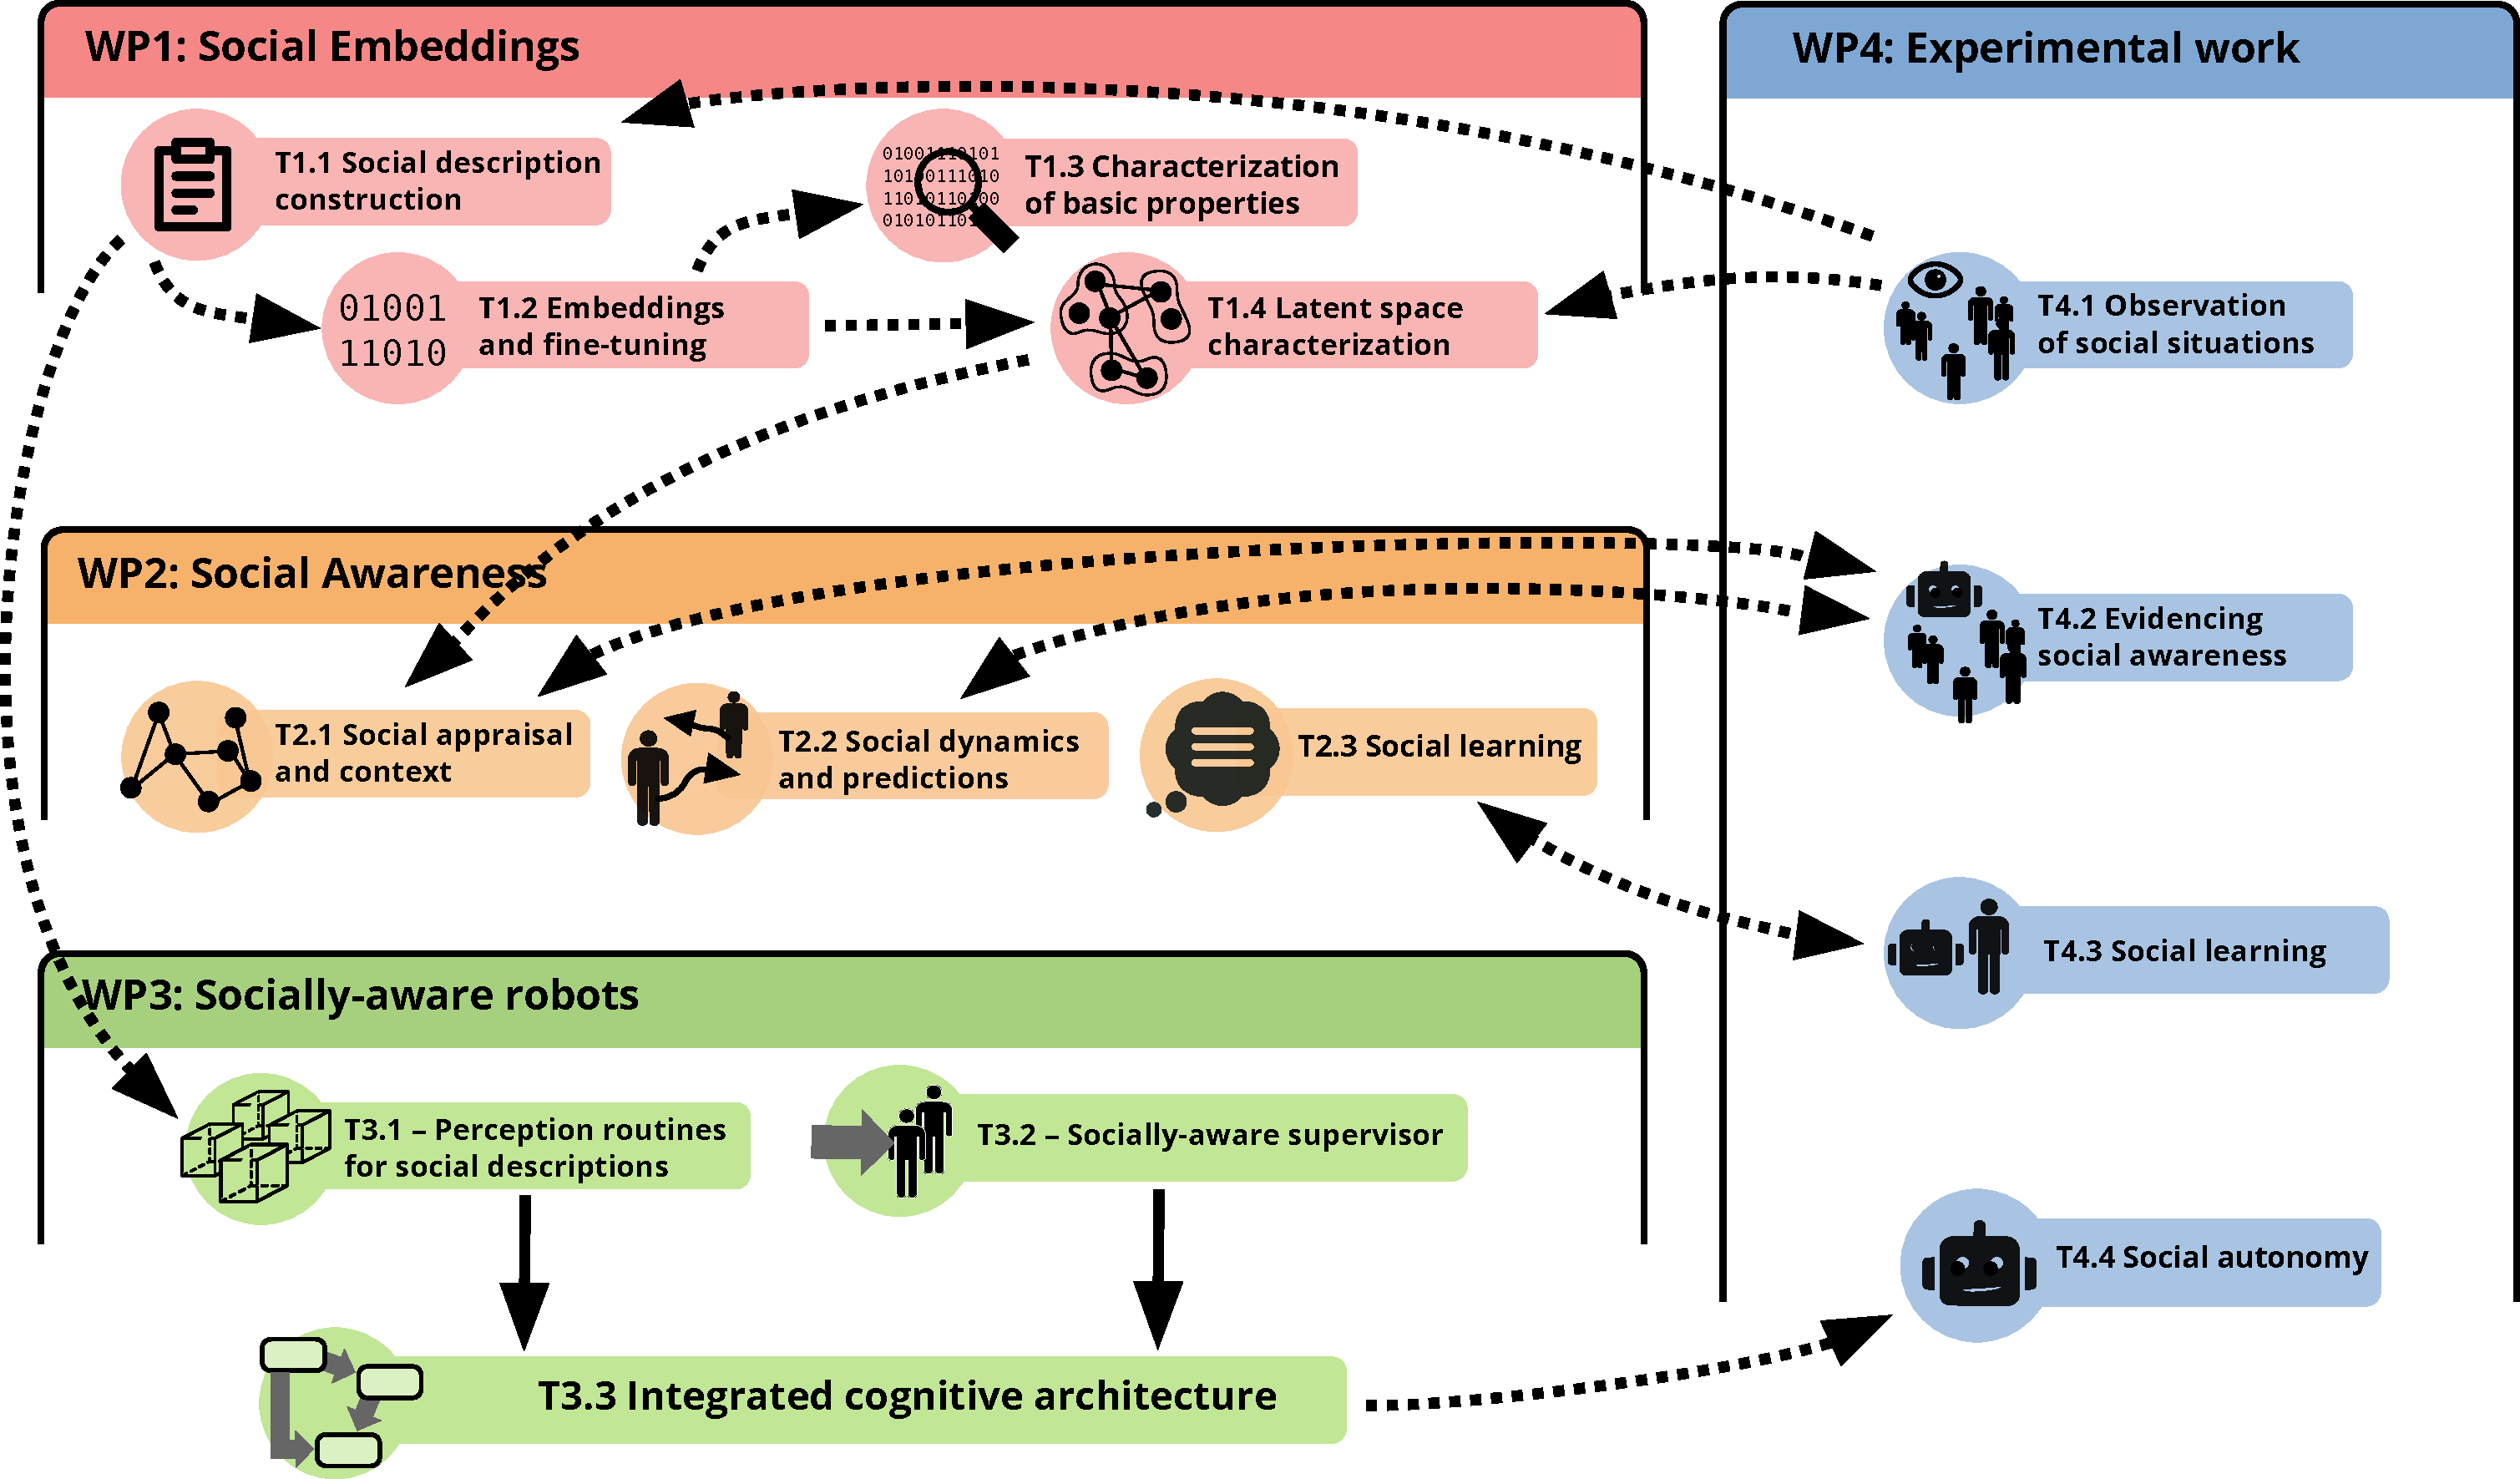
\includegraphics[width=\linewidth]{figs/wps}
\caption{Overview of the workpackages and tasks, and tasks inter-relations.}
\label{fig:wps}
\end{figure}

More specifically, Figure~\ref{fig:wps} gives an overview of the project
workpackages, and their interrelations. Fieldwork plays a central role in the
project, and appears in the centre of the figure. The first important field
deployment is a one-year experiment, taking place at the Bristol science centre
(T1.1). This `public-in-the-loop' experiment is analysed and lead to the
definition of core interaction principles (T1.2). These are in turn translated
into algorithmic models, guiding the social teleology of the cognitive
architecture (T4.1).

This first experiment is immediately followed by two other long-term
experimental deployments: a one-year deployment in one of Bristol's Special
Education Need (SEN) school (T5.1), followed by a one-year deployment at
Bristol's Children's hospital (T5.2). These two additional experiments are both
inputs for WP2 and WP3, and demonstrator for the robot socio-cognitive
architecture (WP4).

Specifically, workpackage WP2 research, develop, and integrate all the components
pertaining to the assessment of the spatio-temporal and social environment of
the robot. Reference interaction situations and the data required to support
this workpackage is directly drawn from the experimental fieldwork that will
take place at the same time in WP1 and WP5. The perceptual capabilities
delivered by WP2 are continuously integrated into the robot's cognitive
architecture (T4.3), iteratively improving the socio-cognitive performances of
the robot.

Workpackage WP3 looks into behaviour generation using machine learning (T3.2)
and non-verbal affective modalities (T3.3). T3.2 is data-intensive, and will use
datasets acquired during the field deployments (T1.1, T5.1, T5.2), as well as
lab-recorded dataset of social interactions. Similar to WP2, the capabilities
built in WP3 are integrated in the robot architecture in T4.3.

In addition to the integration of WP2 and WP3 capabilities, WP4 is also
researching and developing the socio-cognitive drives of the architecture. They
come both from T1.2 (as previously mentioned), and
human-in-the-loop/public-in-the-loop machine learning (T4.2). T4.2, in
particular, is tighly connected to the experimental fieldwork, where the
learning-from-end-users take place.

\subsection{Integration sprints}

\project is a complex project, with numerous interdependencies between tasks.
To ensure the interdependencies are properly understood, and support effective
integration of the outputs of each workpackage, I will organise every 6 months
\textbf{integration sprints} (see Gantt diagram). Integration sprints are
one-week long integration retreat during which the whole \project team gather
and work together to effectively implement and test on the robot the different
components. In addition to providing regular `check points' for the projects,
they also set a stable schedule to deliver project components.

This methodology was adopted in a project the PI previously took part in (FP7
CHRIS project), and had proved at that time to be of great value to ensure
project-wide cohesion and steady progress.

The three integration sprints taking place before the beginning of the
experimental deployments (display as orange circles on the Gantt chart) are of
particular importance, and will be extended to two weeks.

%%%%%%%%%%%%%%%%%%%%%%%%%%%%%%%%%
%% Gantt chart

%\begin{landscape}
\begin{figure}[!ht]
\resizebox{\linewidth}{!}{
    %%%%%%%%%%%%%%%%%
%%
%% Task dependencies
%%
%% Task...        depends on Task...
%% T1.3           T1.1
%% T1.3           T1.2
%% T1.2           T2.2 (user interface)
%% T3.3           T2.3
%%

\definecolor{barcolor}{RGB}{153,204,254}
\definecolor{linkred}{RGB}{165,0,33}
%\renewcommand\sfdefault{phv}
%\renewcommand\mddefault{mc}
%\renewcommand\bfdefault{bc}
\setganttlinklabel{s-s}{START-TO-START}
\setganttlinklabel{f-s}{}
\setganttlinklabel{f-f}{FINISH-TO-FINISH}

%\begin{sidewaysfigure}[!ht]
\begin{figure}[!ht]

%\sffamily
\begin{ganttchart}[
        canvas/.append style={fill=none, draw=black!5, line width=.75pt},
        hgrid style/.style={draw=black!5, line width=.75pt},
        vgrid={*1{draw=black!5, line width=.75pt}},
        %vgrid={*1{black}, *{11}{black!5}}, % doesnt work for some reason
        x unit=.35cm,
        y unit chart=.65cm,
        time slot format=isodate-yearmonth,
        time slot unit=month, % pgfgantt >= 5.0
        %compress calendar, % pgfgantt < 5.0 => overleaf
        title/.style={draw=none, fill=none},
        title label font=\bfseries\footnotesize,
        %title label node/.append style={below=7pt},
        include title in canvas=false,
        bar label font=\mdseries\small\color{black!70},
        %bar label node/.append style={left=2cm},
        bar/.append style={draw=none, fill=barcolor!50},
        bar progress label font=\mdseries\footnotesize\color{black!70},
        group/.append style={fill=barcolor},
        group incomplete/.append style={fill=black},
        group left shift=0,
        group right shift=0,
        group height=.5,
        group peaks tip position=0,
        group label node/.append style={left=.6cm},
        group progress label font=\bfseries\small,
        link/.style={-latex, line width=1.5pt, linkred},
        link label font=\scriptsize\bfseries,
        link label node/.append style={below left=-2pt and 0pt,
        milestone/.append style={circle},
        milestone inline label node/.append style={left=5mm}}
    ]{2021-01}{2025-12}
    
        %\gantttitle[
        %    title label node/.append style={below left=7pt and -3pt}
        %]{Month:\quad1}{1}
        \gantttitlecalendar{year, month} \\
        %\gantttitlelist{0,5,...,60}{1} \\
        %% WP1
        \ganttgroup[]{WP1 \wpOneShort}{2021-01}{2023-12} \\
            \ganttbar[name=WP11]{\textbf{1.1} Conceptual framing \& ethics}{2021-01}{2023-12} \\
            \ganttbar[name=WP12prep,inline,bar/.append style={fill=gray!20}]{preparation}{2021-07}{2021-12}
            \ganttbar[name=WP12exp,inline]{WeTheCurious experiment}{2022-01}{2022-12}
            \ganttbar[name=WP12]{\textbf{1.2} Principles of r-HHI}{2023-01}{2023-06} \\

        %\ganttlink[link type=f-s]{WBS1A}{WBS1B}

        %% WP2
        \definecolor{barcolor}{RGB}{153,2,254}
        \ganttgroup[]{WP2 \wpTwoShort}{2021-01}{2024-12} \\
            \ganttbar[name=WP21]{\textbf{2.1} Situation assessment}{2021-01}{2022-06} \\
            \ganttbar[name=WP22]{\textbf{2.2} Social dynamics}{2022-01}{2023-12} \\
            \ganttbar[name=WP23]{\textbf{2.3} Group dynamics}{2024-01}{2024-12} \\
            \ganttbar[name=WP24]{\textbf{2.4} Social situation assessment}{2022-07}{2024-12} \\

        %\ganttlink[link type=f-s]{WP21}{WP24}
        %\ganttlink[link type=f-s]{WP22}{WP23}

        %% WP3
        \definecolor{barcolor}{RGB}{50,220,134}
        \ganttgroup[]{WP3 \wpThreeShort}{2021-01}{2025-12} \\
            \ganttbar[name=WP31]{\textbf{3.1} Social teleology}{2023-01}{2024-12} \\
            \ganttbar[name=WP32]{\textbf{3.2} Human-in-the-loop policy learning}{2021-07}{2025-06} \\
            \ganttbar[name=WP33]{\textbf{3.3} Integrated cognitive architecture}{2021-01}{2025-06} \\

        %\ganttlink[link type=f-s]{WP12}{WP32}

        %% WP4
        \definecolor{barcolor}{RGB}{244,50,20}
        \ganttgroup[]{WP4 \wpFourShort}{2022-01}{2025-12} \\
            \ganttbar[name=WP41]{\textbf{4.1} Behaviours baselining}{2022-01}{2022-12} \\
            \ganttbar[name=WP42]{\textbf{4.2} Generative behaviours}{2023-01}{2023-12} \\
            \ganttbar[name=WP43]{\textbf{4.3} Non-verbal behaviours}{2023-07}{2025-12} \\


        %% WP5
        \definecolor{barcolor}{RGB}{234,200,20}
        \ganttgroup[]{WP5 \wpFiveShort}{2022-07}{2025-12} \\
            \ganttbar[name=WP51prep,inline,bar/.append style={fill=gray!20}]{preparation}{2022-07}{2022-12}
            \ganttbar[name=WP51]{\textbf{5.1} SEN schools experiment}{2023-01}{2023-12} 
            \ganttbar[name=WP51expl,inline,bar/.append style={fill=gray!20}]{analysis}{2024-01}{2024-06} \\
            \ganttbar[name=WP52prep,inline,bar/.append style={fill=gray!20}]{preparation}{2024-01}{2024-06}
            \ganttbar[name=WP52]{\textbf{5.2} children hospital experiment}{2024-07}{2025-06}
            \ganttbar[name=WP52expl,inline,bar/.append style={fill=gray!20}]{analysis}{2025-07}{2025-12} \\

        %\ganttlink[link type=f-s]{WP41}{WP51}


        %\ganttlink[link type=f-s]{WBS1B}{WBS1C}
        %\ganttlink[link type=f-f,link label node/.append style=left]{WBS1C}{WBS1D}

        \ganttmilestone{\bf\sc Integration sprints}{2021-06}
        \ganttmilestone[milestone/.append style={fill=orange, circle}]{}{2021-11}
        \ganttmilestone{}{2022-06}
        \ganttmilestone[milestone/.append style={fill=orange, circle}]{}{2022-11}
        \ganttmilestone{}{2023-06}
        \ganttmilestone{}{2023-12}
        \ganttmilestone[milestone/.append style={fill=orange, circle}]{}{2024-05}
        \ganttmilestone{}{2024-12}


        % separate years
        \ganttvrule[vrule/.append style={gray, dotted, thin}]{}{2021-12}
        \ganttvrule[vrule/.append style={gray, dotted, thin}]{}{2022-12}
        \ganttvrule[vrule/.append style={gray, dotted, thin}]{}{2023-12}
        \ganttvrule[vrule/.append style={gray, dotted, thin}]{}{2024-12}


        \ganttvrule{start @WeTheCurious}{2021-12}
        \ganttvrule{start @SEN school}{2022-12}
        \ganttvrule{start @Children hospital}{2024-06}

\end{ganttchart}

%\end{sidewaysfigure}
\end{figure}

}
\end{figure}
%\end{landscape}


%%%%%%%%%%%%%%%%%%%%%%%%%%%%%%%%%%%%%%%%%%%%%%%%%%%%%%%%%%%%%%%%%%%%%%%%%%%%%%%%%%%%%%
%%%%%%%%%%%%%%%%%%%%%%%%%%%%%%%%%%%%%%%%%%%%%%%%%%%%%%%%%%%%%%%%%%%%%%%%%%%%%%%%%%%%%%
%%%%%%%%%%%%%%%%%%%%%%%%%%%%%%%%%%%%%%%%%%%%%%%%%%%%%%%%%%%%%%%%%%%%%%%%%%%%%%%%%%%%%%
%%%%%%%%%%%%%%%%%%%%%%%%%%%%%%%%%%%%%%%%%%%%%%%%%%%%%%%%%%%%%%%%%%%%%%%%%%%%%%%%%%%%%%

\subsection{WP1: \textbf{\wpOne}}
\emph{ \textbf{Timeframe:} \textbf{Y1-Y3}; one post-doc (PD1) with expertise in
    deep learning/text embedding; one post-doc (PD2) in data-driven sociology
signal processing/machine learning/cognitive modelling.}

%Objective {\bf O\ref{T1}}.

While I have shown in~\cite{lemaignan2024social} that off-the-shelf Large
Language Models can successfully be applied to compute \emph{proto} social
embeddings, they are still at the level of proof-of-concept.


\paragraph{Fundamental properties}

Fundamental properties of social embeddings, identified
in~\cite{lemaignan2024social}: invariance to pragmatics; social similarity;
continuity.

Hypothesis: social embeddings are a metric of social situations

Data acquisition and groundtruth building

\paragraph{Characterising} Characterising the resulting embedding is largely an open research question. Of
particular interest is the question of the embeddings' latent semantics. For
instance, we can expect that social situations like `two persons chatting
together'; or `a group of three people walking together'; or `one single person
walking towards the robot'; etc. are all semantically distinct, and,
consequently, would belong to distinct regions in the embedding space.
Identifying such clusters to characterize the semantic topology of the embedding
space would enable not only to measure how similar two social situations are,
but also characterize key features of the current situations.  This idea is
related to e.g. the recent investigation by Sun and
Nelson~\cite{sun2023topological} on latent semantics of sentence embeddings.

\paragraph{Fine tuning} their expressiveness could be significantly increased by
fine-tuning. For instance, contrastive-learning-based
fine-tuning~\cite{hadsell2006dimensionality} has shown potential for
instruction-based text embeddings~\cite{canal2022survey}.  Exploring this and
other fine-tuning techniques will be part of the first phase of the project.
Fine-tuning requires appropriately annotated data, whose acquisition I will also
conduct during the project.

\paragraph{Experimental validation} This first workpackage also includes a
focused experimental programme aiming at demonstrating the social representation
capabilities of social embeddings. It is based on protocols originally designed
by Frith and Happé~\cite{frith1994autism} to investigate social representation
in autistic children, that I reframed for social robotics
in~\cite{lemaignan2015mutual}.


%\begin{framed}
%    \textbf{Main outcomes:} A robust, fully characterised model to generate
%    social embeddings;
%
%    \textbf{Timeframe:} \textbf{Y1-Y3}; one post-doc (PD1) with expertise in
%    deep learning/text embedding; one post-doc (PD2) in data-driven sociology
%signal processing/machine learning/cognitive modelling.
%\end{framed}


This work package includes the following tasks:

\begin{enumerate}[label=\textbf{T1.\arabic*}]
    \item Data acquisition of in-the-wild social interactions; annotation of
        social situations; taxonomy of social situations
    \item Construction social embeddings and analysis of their fundamental
        properties (invariance to pragmatics, social similarity, continuity);
    \item Design space of social embedding construction (from indivual facial
        expressions to group formations)
    \item Fine-tuning of LLMs for social embeddings
    \item Characterising of social embeddings (latent semantics, topology of the
        embedding space)
    \item Experimental validation using protocols derived from research on
        autism
\end{enumerate}

\subsection{WP2: \textbf{\wpTwo}}
This work package includes the following tasks:

\begin{enumerate}[label=\textbf{T2.\arabic*}]
    \item{Architecture design and integration}
    \item{Real-time synthesis of social situation descriptions}
    \item{Partial teleoperation for data acquisition}
    \item{Social awareness for robots}
    \item{Modular behaviour executor}
\end{enumerate}

\vspace{1em}
\noindent\emph{Timeframe: Y1-Y3; one PhD student (PHD3) in cognitive
    robotics.}

\subsection{WP4: \textbf{\wpFour}}

Generative neural network for social behaviour production

\project aims at significantly advancing the state of the art in this regard, by
combining two recent techniques: (1) generative neural networks for affective
robot motion generation~\cite{marmpena2019generating,suguitan2020moveae} (with
training data created with an expert choreographer); (2) interactive machine
learning in high-dimensional input/output spaces, where I have shown with my
students promising results for generating complex social
behaviours~\cite{senft2019teaching, winkle2020couch} that fully involve the
end-users~\cite{winkle2018social}. Modulating (1) with the learnt features of
(2), I target a breakthrough in robots' social behaviours generation: the
generation of non-repetitive, socially congruent and transparent social
behaviours (including gestures but also gazing behaviours and facial
expressions).

\begin{oframed}

    \textbf{Main outcomes:} Demonstration that social embeddings enable a new
    class of interactive machine learning application in the social space, by
    offering much richer input representations and features to previously
    explored IML techniques (reinforcement learning, etc).

    \textbf{Timeframe:} \textbf{Y3-Y5}; one PhD student (PHD2) in applied machine
    learning.

\end{oframed}


\subsection{WP5: \textbf{\wpFive}}

\begin{oframed}

    \textbf{Main outcomes:} Demonstration that social embeddings enable a new
    class of interactive machine learning application in the social space, by
    offering much richer input representations and features to previously
    explored IML techniques (reinforcement learning, etc).

    \textbf{Timeframe:} \textbf{Y3-Y5}; one PhD student (PHD2) in applied machine
    learning.

\end{oframed}


This work package includes the following tasks:

\begin{enumerate}[label=\textbf{T5.\arabic*}]
    \item{Refinement of social embeddings for social learning}
    \item{Implementation of an IML-driven behaviour manager}
    \item{Experimental demonstration of interactive learning of social policies}
\end{enumerate}

\vspace{1em}
\noindent\emph{Timeframe: Y3-Y5; one PhD student (PHD2) in applied machine
    learning.}

\subsection{WP6: \textbf{\wpSix}}

\TODO{flesh out, rephrase}
Social embeddings, by enabling artificial systems
to model and reason on their social environment, have the potential of
significantly increase the social competencies of eg robots, also raising
ethical questions.

WP6 aims at establishing the conceptual and ethical framework around the idea of
\emph{robot-supported human-human interactions}. It does so by co-creating
patterns of interaction and norms with the general public, using a unique
combination of ethnographic observations and `crowd-sourced' interaction
patterns.

\begin{framed}
    \textbf{Main outcomes:} A theoretical framework to `think' the role of
    social robots and guidelines to inform policy making (including ethical
    implications); a set of operational \& co-created interaction principles; a
    large dataset of social human-robot interactions

    \textbf{Timeframe:} \textbf{Y3-Y5}; one senior post-doc (PD3)
with background in ethics of technology and responsible innovation.
\end{framed}

This work package includes the following tasks:

\begin{enumerate}[label=\textbf{T6.\arabic*}]
    \item Conceptual framing and ethics of robot-supported social
interactions
    \item \TODO{todo}
\end{enumerate}



\section{WP1: \textbf{\wpOne}}

The basic ambition of \project is to re-investigate the underpinnings of
human-robot interaction by taking a strong human-centered perspective. I frame
this as a shift from \emph{human-robot interaction} to \emph{robot-supported
human-human interactions} (r-HHI). WP1 operationalises this objective in two
tasks: a theoretical contribution, examining the interplay between r-HHI,
responsible AI, and ethics; and a large-scale study to gather public input.

\textbf{T1.1 -- Conceptual framing of r-HHI and ethical framework} 
The first task in WP1 is to research and define the framework that will provide
the conceptual frame around questions like: what role should social robots have?
Where to set the boundaries of artificial social interactions? What does
`ethical-by-design', `responsible-by-design' mean in the context of social
human-robot interactions?

Each of the field experiments (T1.2, T5.1. T5.2) will both \emph{build on} and
\emph{feed into} the framework developed in this task. The work of this task
will be structured around four two-days workshops, spread over the
duration of the project (see Gantt chart). During these workshops, the \project Ethics
Advisory Board, local ethics experts (including the head of the university
ethics committee), and the \project experimental partners (WeTheCurious, the SEN
school network, the Children's hospital) will meet to debate and iterate over
ethics guidelines for responsible long-term social interactions with robots.

\begin{framed}
    {\noindent\bf Main outcomes of T1.1:} a conceptual framework that clarify and
    organise together the questions raised by long-term social interactions;
    initial ethical guidelines for such interactions, aimed at informing future
    policy making.
\end{framed}


\textbf{T1.2 -- Crowd-sourced patterns of robot-supported social
interactions} In order to broadly engage the public with defining what future
robots should do to be perceived as responsible, beneficial, and engaging, T1.2
will create and deploy a novel investigation methodology that I term `experimental
crowd-sourcing'. For one year, in close partnership with the Bristol Science
centre WeTheCurious and its `City Lab' programme, the visitors of the science
centre will be invited to teleoperate a \project robot, with the objective of
interacting and assisting other visitors. The participants will remotely control the
robot through a tablet interface (similar to the setup I created
for~\cite{senft2019teaching} and~\cite{winkle2020couch}), and interviews of both the
teleoperators and the visitors interacting with the robot will be conducted in
parallel, collecting in a structured manner the interaction patterns and social
norms that will emerge over the course of the study. Additional focus groups
will be organised at the science centre to reflect and iterate on these
principles.

During the duration of the study, one researcher will be permanently based at
the science museum, and the museum staff themselves will be trained to
communicate about the aims of the study. Anonymous interaction data (eg, body
postures) will be collected as well, and feed into WP2 and WP3.

\begin{framed}
    {\noindent\bf Main outcomes of T1.2:} a set of crowd-sourced interaction
    patterns and principles, that will inform the long-term social goals of the
    robot (T4.1); a large dataset of social interactions to feed into WP2 and
    WP3.
\end{framed}

%%%%%%%%%%%%%%%%%%%%%%%%%%%%%%%%%%%%%%%%%%%%%%%%%%%%%%%%%%%%%%%%%%%%%%%%%%%%%%%
% WeTheCurious
% 
% - one robot completelty controlled by children, one by adults
% 
% what to learn?
% 
% - when to approach? when to prompt? [example of the salesman/museum facilitator]
% - when is the right time to help/intervene or not? 'child being told off by
% parents -> not the right time!'
% - group interactions -> when to intervene? what about peer-pressure? eg what if
% I tell off one child in front of another?
% - break the barrier for participation. Japanese Journal paper -> facilitating students questions
% - impact on moral norms? what behaviours is acceptable?
% - what role for the robot? another mediator? a peer?
% - what can we do with that 'alien creature'
% 
% - robot taking one child to talk to the museum mediators ("I, robot, am  shy!
% would you come with me?")
% 
% - learning how to adjust behaviour based on personality
% - 'why do I behave like that with that person, and like this with that other
% person?'
% 
% - reinforcement learning instead of human-in-the-loop -> what reinforcement
% signal? engagement
% 
% - the robot that 'take sides': take side against the adults? -> bending in its
% role?
% 
% 
% - social embarassment
% - space for pretence: the robot can adopt an 'artificial role' as long as it is
% possible (accpetable/...) to pretend the robot is


%%%%%%%%%%%%%%%%%%%%%%%%%%%%%%%%%%%%%%%%%%%%%%%%%%%%%%%%%%%%%%%%%%%%%%%%%%%%%%%%%%%%%%
%%%%%%%%%%%%%%%%%%%%%%%%%%%%%%%%%%%%%%%%%%%%%%%%%%%%%%%%%%%%%%%%%%%%%%%%%%%%%%%%%%%%%%
%%%%%%%%%%%%%%%%%%%%%%%%%%%%%%%%%%%%%%%%%%%%%%%%%%%%%%%%%%%%%%%%%%%%%%%%%%%%%%%%%%%%%%
%%%%%%%%%%%%%%%%%%%%%%%%%%%%%%%%%%%%%%%%%%%%%%%%%%%%%%%%%%%%%%%%%%%%%%%%%%%%%%%%%%%%%%

\section{Technical workpackages: WP2, WP3, WP4}

The technical work programme of \project is spread over Workpackages WP2, WP3
and WP4. Figure~\ref{fig:archi} gives an overview of the whole AI engine. WP2
(top) focuses on creating a novel, integrated model of the social environment of
the robot; it will build on the current state of art in spatial modeling,
semantic modeling and interaction history representation, and augment it with
representations of the social dynamics around the robot. WP3 (bottom)
significantly improve upon techniques for non-repetitive, socially-congruent
behaviour production, combining recent advances in generative neural nets, art,
and novel acoustic communication modalities. WP4 (centre) integrates the robot
cognitive capabilities in a new cognitive architecture for long-term social
autonomy. It introduces a novel arbitration mechanism between action policies,
to enable both long-term, goal-driven autonomous behaviours, and direct in-situ
learning from the robot's end-users, to ensure transparency and human oversight.

\begin{figure}[h!]
\centering
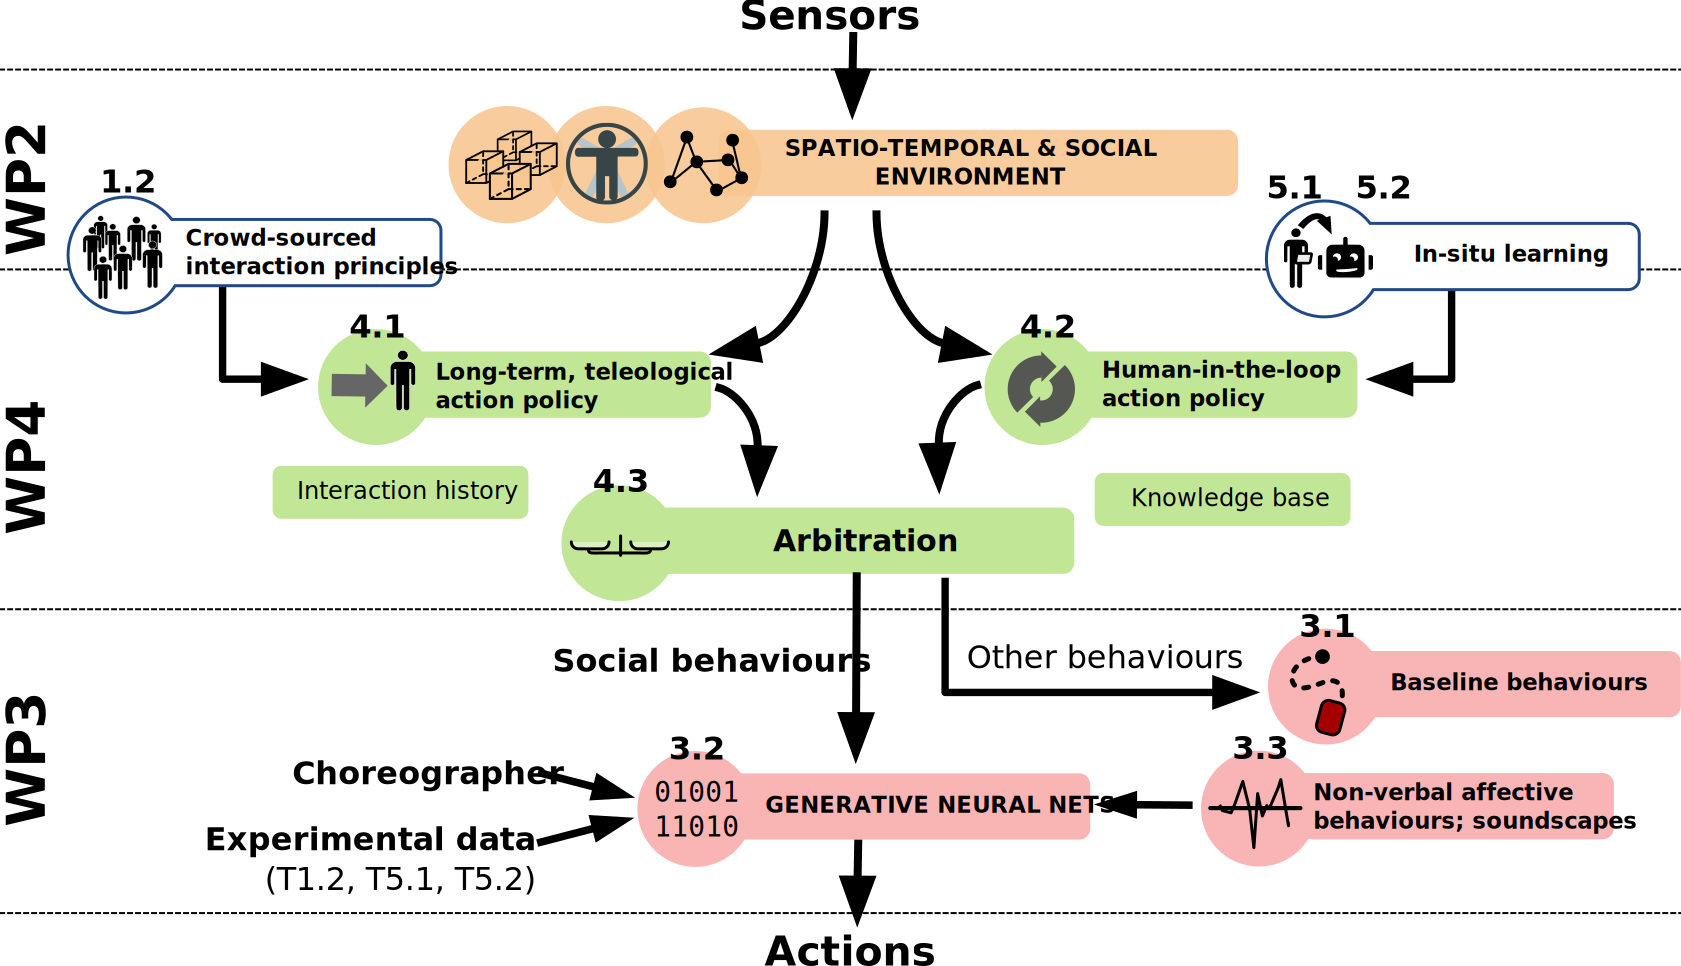
\includegraphics[width=0.8\linewidth]{figs/archi}
\caption{Overview of the AI engine implemented in \project.}
\label{fig:archi}
\end{figure}



%%%%%%%%%%%%%%%%%%%%%%%%%%%%%%%%%%%%%%%%%%%%%%%%%%%%%%%%%%%%%%%%%%%%%%%%%%%%%%%%%%%%%%
%%%%%%%%%%%%%%%%%%%%%%%%%%%%%%%%%%%%%%%%%%%%%%%%%%%%%%%%%%%%%%%%%%%%%%%%%%%%%%%%%%%%%%
%%%%%%%%%%%%%%%%%%%%%%%%%%%%%%%%%%%%%%%%%%%%%%%%%%%%%%%%%%%%%%%%%%%%%%%%%%%%%%%%%%%%%%
%%%%%%%%%%%%%%%%%%%%%%%%%%%%%%%%%%%%%%%%%%%%%%%%%%%%%%%%%%%%%%%%%%%%%%%%%%%%%%%%%%%%%%
\subsection{WP2: \textbf{\wpTwo}}

WP2 will integrate a full representation system for the social environment of
the robot. It builds on existing state of art in \emph{situation assessment} and
\emph{knowledge representation} (T2.1), and extend it to the social sphere
(T2.2, T2.3 and T2.4).

\textbf{T2.1 -- Hybrid situation assessment and knowledge representation}
Knowledge representation and grounding is a fundamental building block for
cognitive architectures~\cite{lemaignan2017artificial,beetz2010cram}. This task
builds on existing work on symbolic knowledge representation
(eg~\cite{tenorth2009knowrob} or my own work~\cite{lemaignan2010oro}) and my
work on situation assessment~\cite{lemaignan2018underworlds} (that includes for
instance object recognition and physics
simulation~\cite{sallami2019simulation}), to create a coherent system of
representations for the cognitive architecture that extends the \sc{underworlds}
spatio-temporal representation tool~\cite{lemaignan2018underworlds} with
symbolic and hybrid (like \emph{conceptors}~\cite{jaeger2014controlling})
representations capabilities.

\begin{framed}
    {\noindent\bf Main outcomes of T2.1:} an extensible multi-modal
    software platform, that tracks and represents the spatio-temporal
    environment of the robot (including the locations and objects in the robot
    vicinity).
\end{framed}

\textbf{T2.2 -- Multi-modal human model}
This task focuses on the acquisition, processing and modelling of social
signals~\cite{gunes2017automatic} to build a multi-modal model of the humans
in the robot's vicinity. I have recently introduced a dataset of social
interaction~\cite{lemaignan2018pinsoro} that enables for the first time a
quantitative, data-driven investigation of social dynamics. Promising initial
results led me to uncover three latent constructs that underpin social
interactions~\cite{bartlett2019what}. This dataset and the related methodologies
on data-driven social modeling will form the basis of this task, with additional
data of natural interactions collected during T1.2.

\begin{framed}
    {\noindent\bf Main outcome of T2.2:} A data-driven social signal processing
    pipeline to model the surrounding humans.
\end{framed}

\textbf{T2.3 -- Interaction and group dynamics} Building on T2.2, T2.3
investigates the automatic understanding and modelling of group-level social
interactions~\cite{tapus2019perceiving}, including
$f$-formations~\cite{marshall2011using}, sociograms (as done
in~\cite{garcia2016hybrid} for instance), and inter-personal
affordances~\cite{pandey2013affordance}. This task builds on literature on on
social dynamics analysis (eg~\cite{durantin2017social,jermann2009physical,
martinez2019collocated}) to apply it to real-time social assessment by a robot,
itself embedded into the interaction.

\begin{framed}
    {\noindent\bf Main outcome of T2.3:} the software pipeline required for the automatic analysis of social
    dynamics at group-level, able to model in real-time the social context
    of the robot.
\end{framed}


\textbf{T2.4 -- Social situation assessment} In T2.4, I integrate the social
cues from T2.2 and T2.3 into the representation platform of T2.1. It will result in
a socio-cognitive model of the social environment of the robot that I term
\emph{social situation assessment}. It effectively extends the representation
capabilities of T2.1 to the social sphere, and covers the development of a
complete social assessment pipeline, from social signal perception (like
automatic attention tracking, face recognition, sound localisation, etc.) to
higher-level socio-cognitive constructs, including group dynamics and
perspective taking~\cite{flavell1992perspectives} (as I previously framed
in~\cite{lemaignan2015mutual, dillenbourg2016symmetry}).

Part of this task, I will also construct a \emph{social embedding} of the robot:
a compact, low-dimensional representation of the full social environment, that
can be easily integrated with the machine learning algorithms developed in WP3
and WP4.

A focused experimental programme accompanies T2.4, to demonstrate (in relative
isolation) the resulting socio-cognitive capabilities. I will implement a subset
of the experimental protocols identified by Frith and
Happé~\cite{frith1994autism} to investigate theory of mind with autistic
children, as it offers an excellent experimental framework for social
robotics~\cite{lemaignan2015mutual} for this work.

%Experimental protocols in research on autistic spectrum disorders are often
%striking by their apparent straightforwardness because of the careful choice of
%interaction modalities: since autistic children frequently exhibit impairments
%beyond social ones (such as motor or linguistic ones), the experiments must be
%designed such that they require only basic cognitive skills beyond the social
%abilities that are tested. The Sally and Anne task, for instance, requires the
%observing child to be able to visually follow the marble, to remember the true
%location of the marble, to understand simple questions (``Where will Sally look
%for her marble?'' in Baron-Cohen's protocol~\cite{baron1985does}) and eventually
%to give an answer, either verbally or with a gesture -- the two first points
%being actually explicitly checked through questions: ``Where is the marble
%really?'' (reality control question) and ``Where was the marble in the
%beginning?'' (memory control question).
%
%Likewise, current social robots have limited cognitive skills (no fast yet fine
%motor skills, limited speech production and understanding, limited scene
%segmentation and object recognition capabilities, etc.) and such tasks
%that effectively test a single cognitive skill (in this case, mentalizing) in
%near isolation are of high relevance for experimental social robotics.
%
%\begin{table}[h]
%    \centering
%    \begin{tabular}{p{0.4\linewidth}p{0.5\linewidth}}
%        \toprule
%        No mentalizing required           & Mentalizing required          \\
%        \midrule
%        Ordering behavioural pictures     & Ordering mentalistic pictures~\cite{baron1986mechanical} \\
%        Understanding see                 & Understanding know~\cite{perner1989exploration}            \\
%        Protoimperative pointing          & Protodeclarative pointing~\cite{baron1989perceptual}     \\
%        Sabotage                          & Deception~\cite{sodian1992deception}                     \\
%        False photographs                 & False beliefs~\cite{leslie1992domain}                 \\
%        Recognizing happiness and sadness & Recognizing surprise~\cite{baron1993children}          \\
%        Object occlusion                  & Information occlusion~\cite{baron1992out}         \\
%        Literal expression                & Metaphorical expression~\cite{happe1993communicative}       \\
%        \bottomrule
%    \end{tabular}
%    \caption{\small Tasks requiring or not mentalizing to pass, listed by Frith and Happé in~\cite{frith1994autism}}
%    \label{mentalizing-tasks}
%\end{table}
%
%Frith and Happé's list (Table~\ref{mentalizing-tasks}) is in that regard
%especially interesting in that it mirrors pairs of task (ones which do not
%require mentalizing with similar ones which do require mentalizing), thus
%providing control tasks.  \emph{Object occlusion} vs.~\emph{Information
%occlusion} is one example of a (pair of) task(s) which evidence
%representation-level perspective taking through \emph{adaptive deception}:
%during a simple game, the experimenter adapts its strategy
%(deceptive/non-deceptive behaviour) to the representation skills of its child
%opponent. The experimental setting is derived from the penny-hiding game
%protocol originally proposed by Oswald and Ollendick~\cite{oswald1989role} and
%replicated and extended by Baron-Cohen in~\cite{baron1992out}, who describes it
%as a two-person game in which the subject is actively involved, either as a
%guesser or as a hider. The hider hides the penny in one hand or the other, and
%then invites a guess. The game is repeated several time before switching the
%roles. Baron-Cohen proposes a specific index to rate the level of the players
%based on the idea of \emph{information occlusion}: minimally, the hider must
%ensure \emph{object occlusion} (the penny must not become visible to the
%guesser), while good hiders, with representation-level perspective taking
%skills, develop strategies (like random hand switching or deictic hints at the
%wrong hand) to prevent the guesser to find the penny (\emph{information
%occlusion}). One could imagine a similar protocol adapted to robotics: the robot
%would play the role of the experimenter, adapting on-line its
%behaviour to what it understands of the perspective taking capabilities of the
%children, and would consequently require \emph{second-order},
%\emph{representation-level} perspective taking from the robot.

\begin{framed}
    {\noindent\bf Main outcome of T2.4:} a novel cognitive sub-system for social
    situation assessment, released as an open-source set of integrated ROS
    modules. This tool will enable the robot to represent its physical and
    social environment, and perform queries about it, including queries about
    past events (temporal model) and queries requiring higher socio-cognitive
    perceptual capabilities like perspective taking.
\end{framed}





%%%%%%%%%%%%%%%%%%%%%%%%%%%%%%%%%%%%%%%%%%%%%%%%%%%%%%%%%%%%%%%%%%%%%%%%%%%%%%%%%%%%%%
%%%%%%%%%%%%%%%%%%%%%%%%%%%%%%%%%%%%%%%%%%%%%%%%%%%%%%%%%%%%%%%%%%%%%%%%%%%%%%%%%%%%%%
%%%%%%%%%%%%%%%%%%%%%%%%%%%%%%%%%%%%%%%%%%%%%%%%%%%%%%%%%%%%%%%%%%%%%%%%%%%%%%%%%%%%%%
%%%%%%%%%%%%%%%%%%%%%%%%%%%%%%%%%%%%%%%%%%%%%%%%%%%%%%%%%%%%%%%%%%%%%%%%%%%%%%%%%%%%%%
\subsection{WP3: \textbf{\wpThree}} 


Mirroring WP2's focus on understanding the social interactions, WP3 addresses the
question of social behaviour \emph{generation}: how to create natural
behaviours, engaging over a sustained period of time (eg not simply picking
scripted behaviours from a library, that are rapidly perceived as repetitive).

Using on-board speech recognition (Mozilla DeepSpeech), the robots will be able to understand and
record the textual transcription of the what the end-users say (in WP5, mostly
children). The robots themselves are however purposefully designed \emph{not} to
speak, using instead non-verbal communication mechanisms (non-verbal utterances
using sounds, gaze, joint attention, expressive motions, etc). This is a
critical interaction design choice, that ensures we can more effectively manage
what cognitive capabilities are ascribed to the robot by the users (expectation
management).  \project seeks however to significantly push forward the
state-of-the-art of behaviour generation for robots, both in term of technique to
generate the behaviours, and in term of the nature of the non-verbal behaviours.


\textbf{T3.1 -- Behavioural baseline}
T3.1 establishes a baseline for behaviour
generation, by surveying and implementing the current state of the art. In
addition to traditional approaches like behaviour libraries, this will cover
techniques like curiosity-driven behaviours~\cite{oudeyer2005playground},
Learning from Demonstration~\cite{billard2008robot, argall2009survey},
human-in-the-loop action policy learning~\cite{senft2016sparc,
senft2019teaching}. This baseline will enable early in-situ experimental
deployments (WP5), while also provide a comparison point for T3.2.

Using activity switching to support long term engagement with diabetic children~\cite{coninx2016towards}

\begin{framed}
    {\noindent\bf Main outcomes of T3.1:} A set of base behaviours for the robot, both
    social (like gesture,  gaze), and generic (like navigation in crowded
    space). This task focuses on providing a working set of robot behaviours
    early in the project, using existing state of art.
\end{framed}


\textbf{T3.2 -- Generative neural network for social behaviour production}

Producing non-repetitive social behaviours is an open research question. I aim
at significantly advancing the state of the art in this regard, by combining two
recent techniques: (1) generative neural networks for affective robot motion
generation~\cite{marmpena2019generating,suguitan2020moveae}; (2) interactive
machine learning in high-dimensional input/output spaces, where I have shown
with my students promising results for generating complex social
behaviours~\cite{senft2019teaching, winkle2020couch} that fully involve the
end-users~\cite{winkle2018social}.

In~\cite{suguitan2020moveae}, a Generative Adversarial Network (GAN) is trained
to generate expressive motions; the generation being modulated by a feature
encoding an emotion. I will extend this idea in two ways: (1) I will train the GAN on multiple
interaction modalities (motions, but also facial expressions, gaze, sounds) with
a dataset co-created with a choreographer: during one month, a choreographer from the
puppetering company RustySquid (with whom we have had several collaborations)
will join the lab and remotely `puppet' the robot while interacting with the lab
members. The aim will be to collect a large amount of data to train the GAN
from, effectively creating a new multi-modal `grammar' for the robot expression.
(2) Instead of using emotions to modulate the generation stage, I will use the
social embedding constructed in T2.4: the generated behaviours will be shaped by
the current social state of the interaction.

%
%\begin{wrapfigure}{l}{7cm}
%    \centering
%    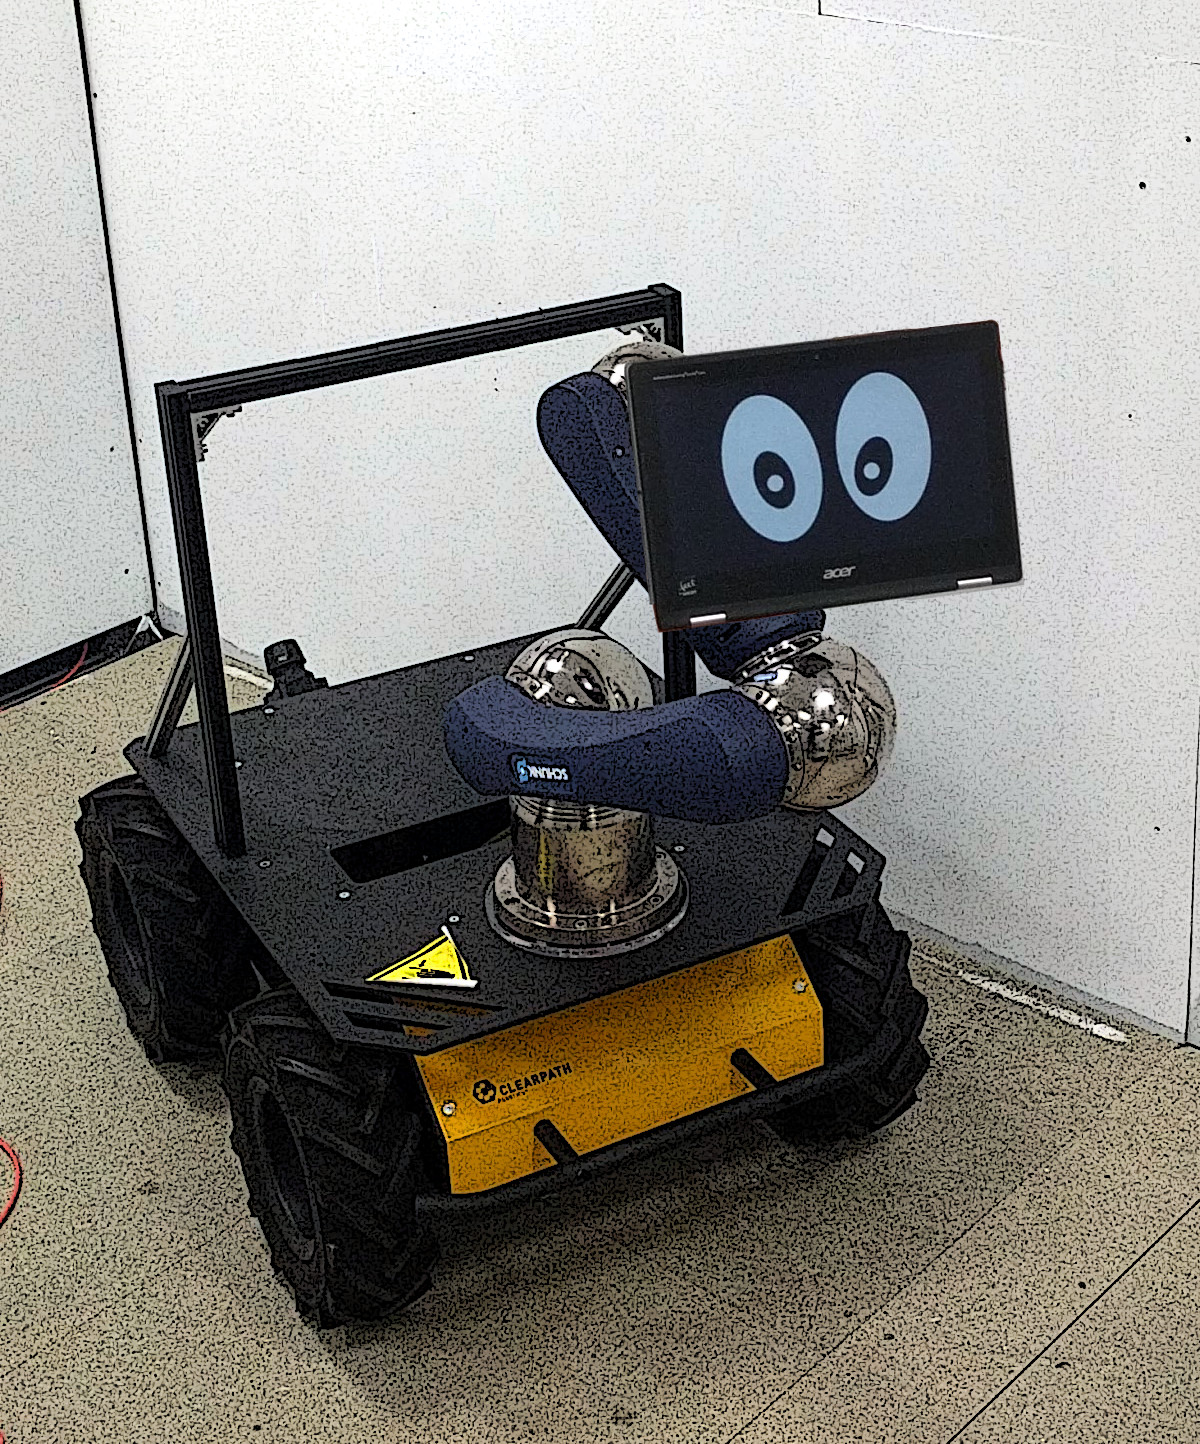
\includegraphics[width=\linewidth]{figs/husky.jpg}
%    \caption{\label{fig:robot}
%    Provisional appearance of the \project robot that we will use to collect
%    data. A tablet, displaying facial animations, is mounted on a robotic arm.
%    It can freely orient its `gaze' and use expressive movements. The mobile
%    base (a Segway Husky) can autonomously navigate in the various parts of the
%    BRL open-space}
%\end{wrapfigure}

%Designing behaviours that
%enable sustained, long-term engagement in a social human-robot interaction is
%essentially an open research question. Three main approaches to social
%behaviours generation exist today: \emph{user-induced}, where the end-user
%interacts with the robot and ascribes (knowingly or not) complex behaviours to
%the machine, while in reality the robot's behaviours are simple and non-goal
%oriented (eg generating a noise or a small movement when being touched). This
%has been used to great effect in therapy robots, for instance (eg Paro).
%\emph{Off-the-shelf behaviours}, where the robot relies on a set library of
%behaviours (that might be individually relatively complex). The approach can
%elicit a strong initial social response from the user, but this social response
%tends to vanish rapidly once the `tricks' of the robot have been all discovered
%and become repetitive.  Besides, as the robot does not typically maintain a
%long-term socio-cognitive plan of the interaction, the behaviours are typically
%perceived as fun, yet pointless. This is often observed in toy-like robots (eg
%Vector, Dot \& Dash). Finally, many social robots avoid altogether the problem
%of generating behaviours by simply offering to the end-user control over
%\emph{low-level behaviours} (eg, control of the joints of the robot). This means
%that, even when the robot has relatively powerful social perception capabilities
%(like recognising people and voice), no real social behaviours is generated.
%
%None of these three approaches are satisfactory, and indeed, no approach to date
%has been able to engage human users in long-term, sustained interactions.
%
%
%
%
%At a time where companion robots are coming to the market, one important
%question remains fully open: how to design robot behaviours that foster
%lasting engagement? A vast body of academic literature identifies that
%robots evoke an initial phase of high user engagement (the
%\emph{novelty} phase) that vanishes as the user realises that the robot
%is actually quite predictable and repetitive. The \emph{agency}
%initially ascribed by the user to the robot quickly
%fades~\cite{lemaignan2014dynamics}, leading to critical user disengagement from the technology.
%
%
%The (often limited) library of behaviours available to the robot is
%often cited as a key factor in causing this issue. However, another,
%more profound issue affecting long term engagement with robot companions
%is the question of \emph{purpose.} Without clear \emph{purpose}, social
%robot companions can lack \emph{usefulness}. Indeed, robot
%\emph{companions} might not have explicit goals that would dictate or
%motivate their behaviours: they aim at providing a social presence, a
%social comfort, as cats or dogs would do, without necessarily being
%goal-oriented.
%
%Recent attempts -- and failures -- to convert social robotics research
%into commercial platforms (Jibo, Kuri and most recently Anki's Cozmo and
%Vector robots) reflect exactly this, with reasons for their failure
%typically citing an under-delivery of the user experience they promised,
%and/or the lack of a `real need' to justify their price point. The
%\project project addresses these two key issues by:
%
%\begin{enumerate}
%\def\labelenumi{\arabic{enumi}.}
%\item
%  Taking inspiration from human-pet relationships which also have no
%  explicit \emph{purpose} beyond their potential for enjoyable,
%  \emph{affective} interactions;
%\item
%  Working with creative professionals who excel at storytelling and
%  emotional engagement to overcome the problems in sustaining
%        engagement, as proposed by Hoffman~\cite{hoffman2019anki}
%\item
%  Blending these two sources of inspiration using a radically novel
%  combination of immersive teleoperation and machine learning.
%\end{enumerate}
%
%The project is \emph{not} about replicating a pet's behaviour per se. It
%is instead about identifying, modeling and automatically generating the
%social behaviours required to recreate pet-like social dynamics between
%robots and humans, drawing inspiration from ethology (Stanton, Sullivan,
%and Fazio 2015). Using animal behaviours to inform the design of robots
%is not new, the most remarkable example being the Sony AIBO robot dog,
%whose behaviours were directly designed around those of actual dogs
%(Arkin et al. 2003). However, to go beyond the repetitive interactions
%associated with such robots, we propose to employ a creative
%professional to actively participate in design and automation of \project
%behaviour. The concept of using creative professionals to `teach' social
%robot behaviour is not new either (Knight and Gray 2012), however it is
%only recent advances in human-in-the-loop, online machine learning that
%make this type of real-time `social training' a feasible approach to
%generating and automating engaging social behaviours (Senft et al.
%2019).
%
%Our project has the following goals, addressed by the workplan presented
%below:
%
%\begin{enumerate}
%\def\labelenumi{\arabic{enumi}.}
%\item
%  assemble a non-anthropomorphic social robot that can autonomously
%  navigate in a complex and living lab environment, taking inspiration
%  from ethology to inspire the robot's behaviour;
%\item
%  develop an immersive teleoperation system, enabling a creative
%  professional to `take control' of the robot (i.e.~puppet the robot) in
%  a completely intuitive way (using whole body motion tracking);
%\item
%  record (and make publicly available) a large dataset of social
%  behaviours (created through immersive teleoperation) that foster
%  long-term social and affective engagement. The dataset will also
%  include the social \emph{signals} implicitly used by the puppeteer to
%  drive his/her choice of actions (recorded through eg eye-tracking);
%\item
%  using machine learning, map these social signals (input state) to the
%  robot behaviours (output state) such that the robot can operate
%  autonomously.
%\end{enumerate}
%
%A creative professional (puppeteer, dancer or comedian --
%corresponding financial compensation is budgeted) will join the group.
%First she/he will take part to a one-week co-design workshop (4) aiming
%at finalising the immersive teleoperation controller and the behaviours
%of the robot. Then, she/he will interact for about 4 hours a day during
%a month, with the BRL lab members (200+ researchers). She/he will do so
%by remotely operating the robot (5) from an (out-of-sight) control room
%(the BRL CAVE room). The aim will be for the puppeteer to pro-actively
%engage with people in the lab, attempting to engage in \emph{social,
%affective} interactions. This will be achieved by creating/inventing
%in-situ a new `grammar' of social behaviour, loosely inspired by those
%of cats and other pets. These interactions will be fully recorded
%(including eye-tracking on the puppeeter) (6), in order to create a
%unique dataset of complex social interactions, suitable for machine
%learning. The PI has already extensive experience in recording such
%datasets (see (Lemaignan et al. 2018) for instance).
%
%%%\begin{wrapfigure}[17]{l}{8cm}
%%\begin{figure}
%%    \centering
%%    
\includegraphics[width=0.8\paperwidth]{figs/dev.pdf}
%%    \caption{\label{fig:support}
%%    Social behaviours will be learned from immersive `puppetering' of the
%%    robot, performed by a professional actor. The `puppetering' takes place
%%    in a CAVE (or VR) environment, where what the robot `sees' and `hears'
%%    is streamed live}
%%\end{figure}
%%%\end{wrapfigure}
%
%Over the following four months, a deep neural network will be designed
%and trained (7) for the regression task of generating continuous social
%behaviours from perceived social signals. In parallel, a software
%controller will be developed (8) to enable generic autonomous
%capabilities (like autonomous navigation) for which the BRL has
%extensive expertise.
%
%Finally, the last four months will be dedicated to in-situ testing of
%the autonomous system (9). We will seek to conduct a large scale study
%within the lab, over a period of several weeks. For this study, the
%robot is expected to be fully autonomous. However sufficient amount of
%time is planned for additional iterations on the development of the
%robot controller if deemed necessary. We aim at publishing the results
%of this main study shortly after the end of the one-year period.

\begin{framed}
    {\noindent\bf Main outcomes of T3.2:} a generative neural network able to produce
    non-verbal yet multi-modal social behaviours. They will combine expressive gestures, gazing
    behaviours, facial expressions, and expressive sounds.
\end{framed}


\textbf{T3.3: Non-verbal behaviours and robot soundscape}

%\begin{figure}[!htbp]
%\centering
%    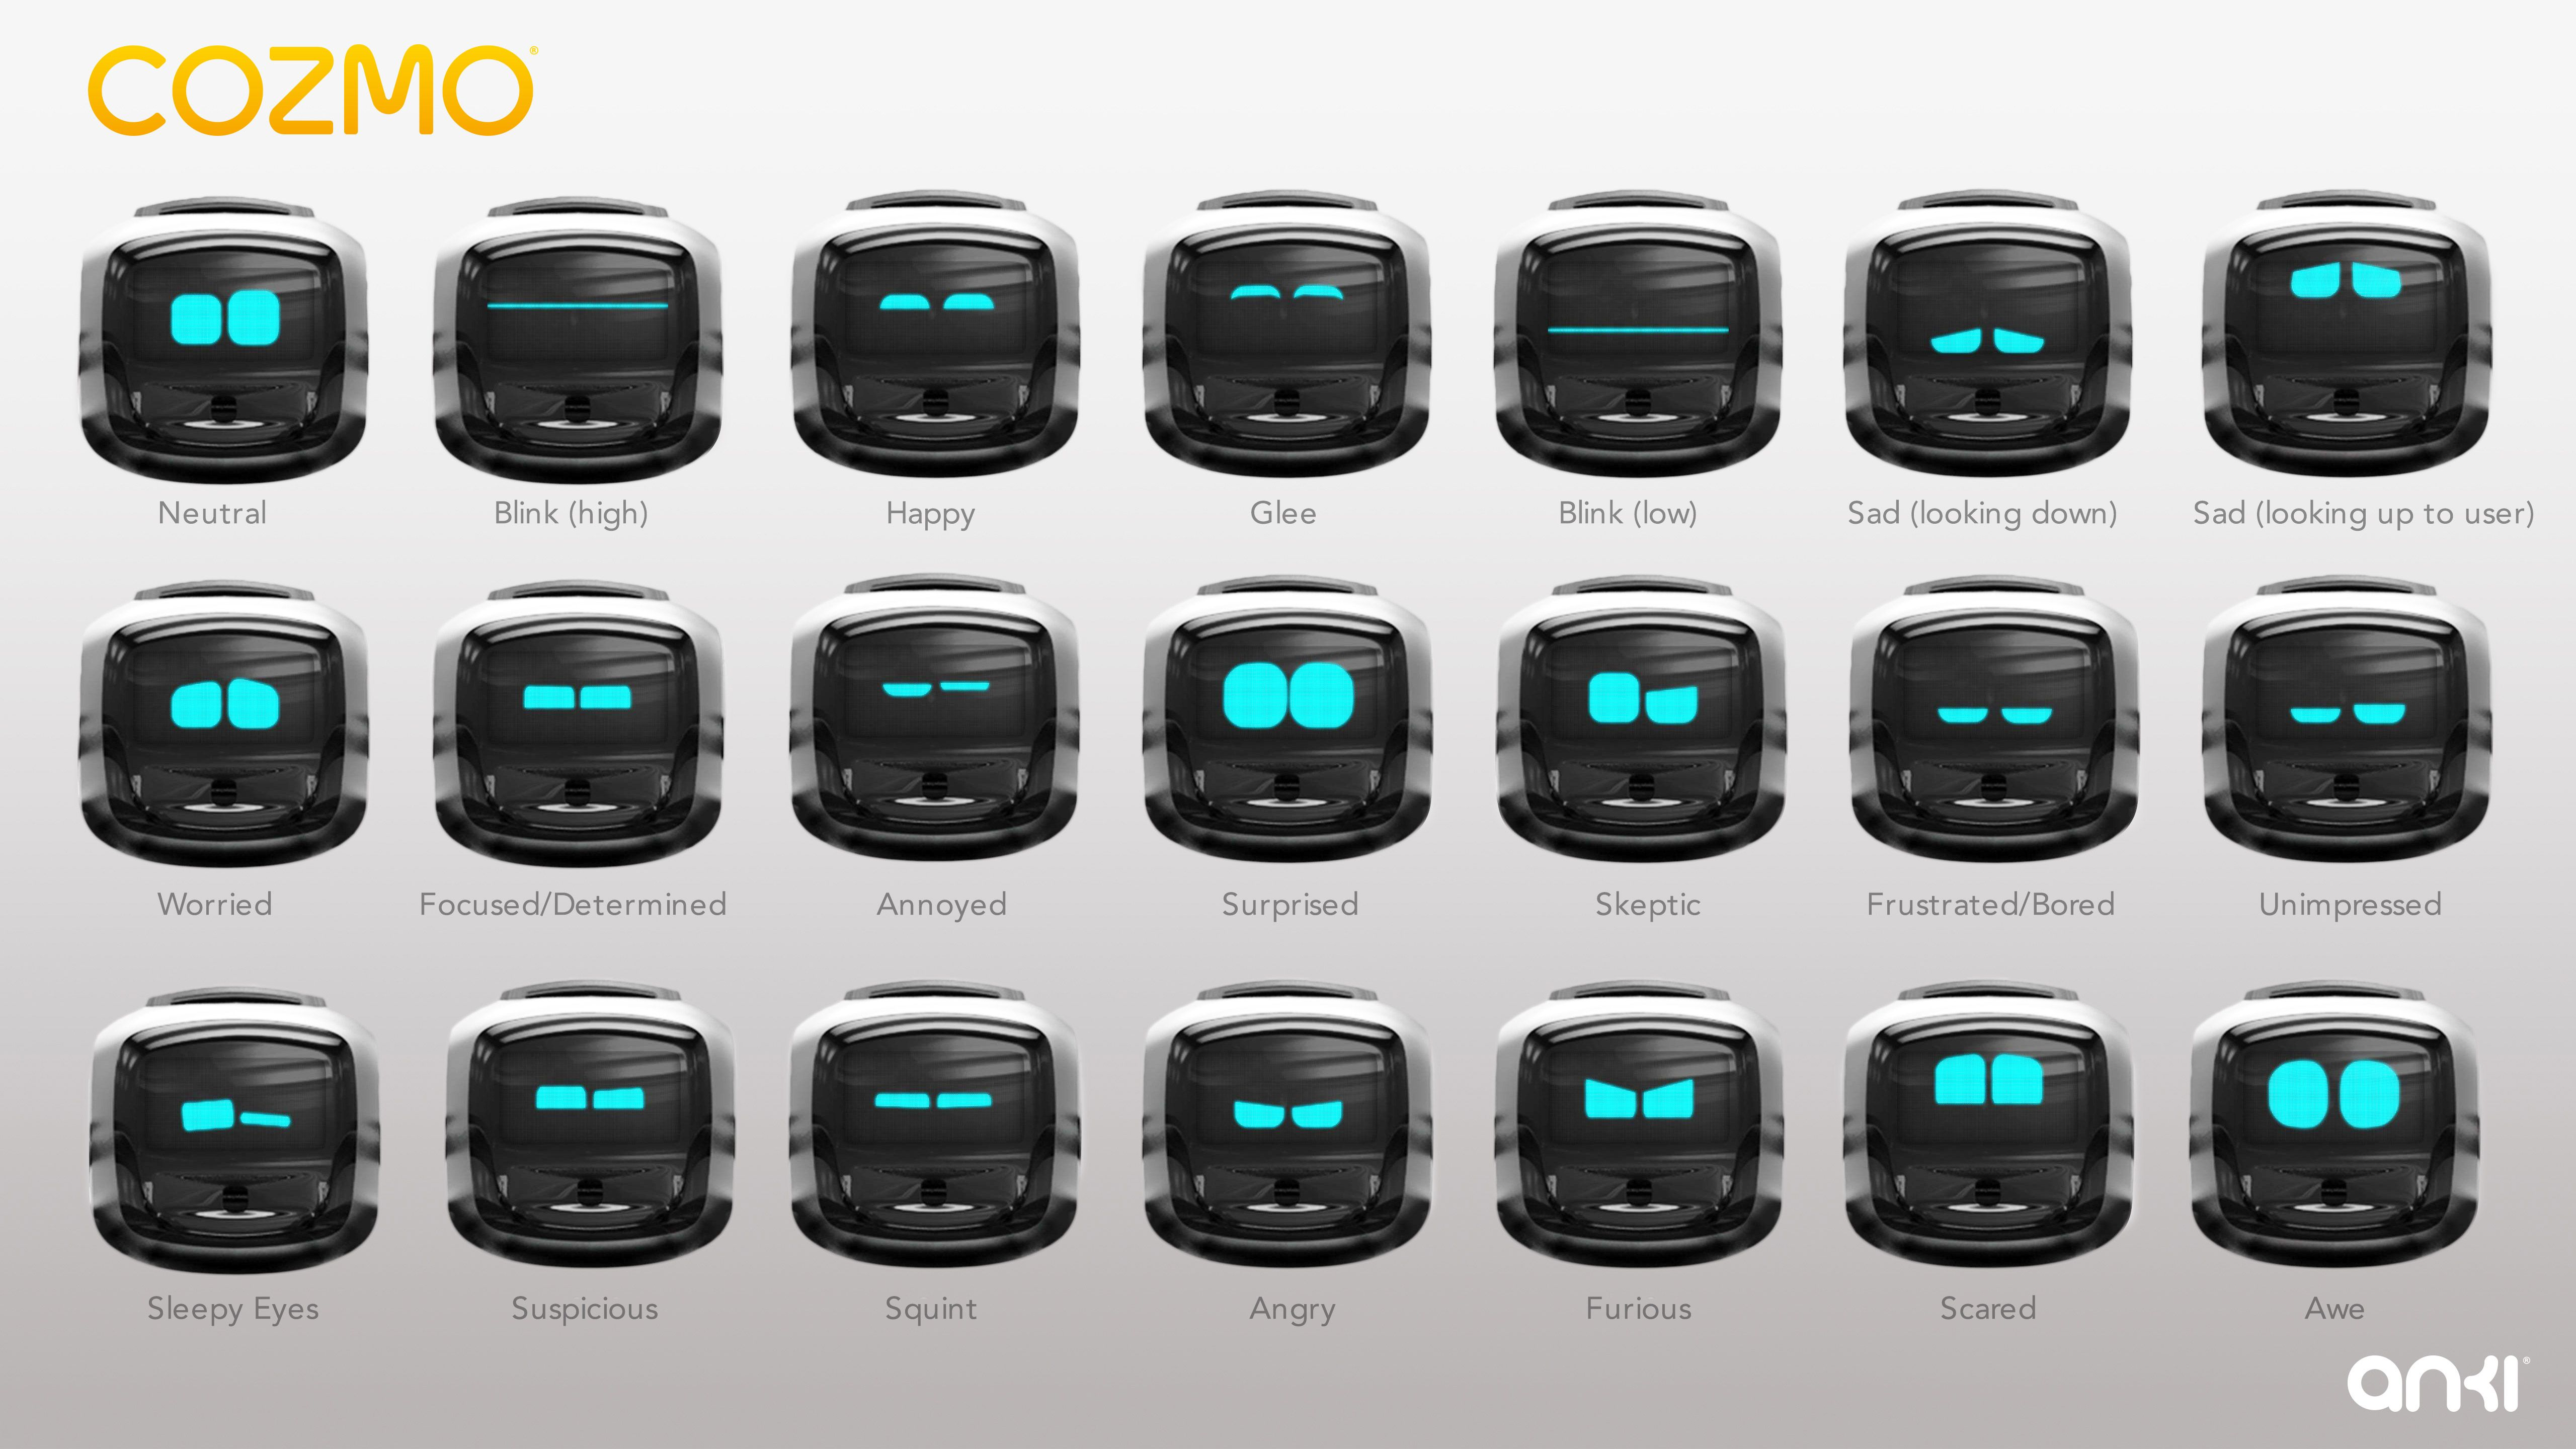
\includegraphics[width=0.7\textwidth]{figs/cozmo-expression-sheet.jpg}
%\caption{Cozmo facial expressions}
%\end{figure}

In task T3.3, we introduce a novel non-verbal interaction modality for robots,
based on soundscapes: soundscapes are about creating a sound environment that
reflects a particular situation; they also have been shown to be an effective
intervention technique in the context special needs treatments
(eg~\cite{greher2010soundscape}). The soundscapes that we will create, are
`owned' by the robot, and it can manipulate it itself, eg to create an
approachable, non-threatening, non-judgmental, social interaction context, or to
the establish the interaction into a trusted physical and emotional safe-space
for the children.

\begin{framed}
    {\noindent\bf Main outcomes of T3.3:} the development and implementation of
    soundscapes, a novel non-verbal interaction modality, integrated with the
    behaviours production of T3.2.
\end{framed}



%%%%%%%%%%%%%%%%%%%%%%%%%%%%%%%%%%%%%%%%%%%%%%%%%%%%%%%%%%%%%%%%%%%%%%%%%%%%%%%%%%%%%%
%%%%%%%%%%%%%%%%%%%%%%%%%%%%%%%%%%%%%%%%%%%%%%%%%%%%%%%%%%%%%%%%%%%%%%%%%%%%%%%%%%%%%%
%%%%%%%%%%%%%%%%%%%%%%%%%%%%%%%%%%%%%%%%%%%%%%%%%%%%%%%%%%%%%%%%%%%%%%%%%%%%%%%%%%%%%%
%%%%%%%%%%%%%%%%%%%%%%%%%%%%%%%%%%%%%%%%%%%%%%%%%%%%%%%%%%%%%%%%%%%%%%%%%%%%%%%%%%%%%%
%%%%%%%%%%%%%%%%%%%%%%%%%%%%%%%%%%%%%%%%%%%%%%%%%%%%%%%%%%%%%%%%%%%%%%%%%%%%%%%%%
%%%%%%%%%%%%%%%%%%%%%%%%%%%%%%%%%%%%%%%%%%%%%%%%%%%%%%%%%%%%%%%%%%%%%%%%%%%%%%%%%
%%%%%%%%%%%%%%%%%%%%%%%%%%%%%%%%%%%%%%%%%%%%%%%%%%%%%%%%%%%%%%%%%%%%%%%%%%%%%%%%%
%%%%%%%%%%%%%%%%%%%%%%%%%%%%%%%%%%%%%%%%%%%%%%%%%%%%%%%%%%%%%%%%%%%%%%%%%%%%%%%%%
\subsection{WP4: \textbf{\wpFour}}

WP4 design and implement on the R1 robot the principled cognitive architecture
that binds together the socio-cognitive perceptual capabilities of the robot
(WP2), with its action production mechanisms (WP3).

\textbf{T4.1 -- A social teleology for robots}
\emph{Teleological systems} (ie goal-driven) has been investigated in robotics
for being a way of providing long-term drives to an autonomous robot. This has
been successfully applied to curiosity-driven robots~\cite{oudeyer2005playground} or motor babbling in infant-like
robots~\cite{forestier2017unified}, but only for relatively simple cognitive
systems. This task's objective is to define and implement a novel \emph{social teleology} that would
algorithmically encode long-term social goals into the robot. This will directly
build from the results of WP1, where interaction principles for social robots
are experimentally uncovered.

\begin{framed}
    {\noindent\bf Main outcomes of T4.1:} the algorithmic translation of WP1's
    interaction principles in long-term social goals for the robot, eg a
    long-term, socially-driven action policy for the robot.
\end{framed}

\textbf{T4.2 -- Learning from humans to achieve `by-design' responsible \&
trustworthy AI}
Building on my recent, promising results on human-in-the-loop
social learning~\cite{senft2019teaching,winkle2020couch}, this task
implements the learning mechanics (including the bi-directional interface
between the human teacher and the robot) to allow human end-users to
teach the robot domain-specific (at school, at the hospital) social policies,
following the methodology and the interactive reinforcement learning approach I
developed with my students in~\cite{senft2017supervised}.

In addition, this task will study through qualitative methods (thematic
interviews and questionnaires) how human-in-the-loop machine learning enables a more
trustworthy AI system, by involving the end-users in the creation of the robot
behaviours, thus offering a level of behavioural transparency to the end-users.

\begin{framed}
    {\noindent\bf Main outcomes of T4.2:} a human-in-the-loop reinforcement
    learning paradigm, suitable for in-situ teaching of the robot by the
    end-users themselves.
\end{framed}

\textbf{T4.3 -- Integrating a socially-driven architecture for long-term interaction}
This task builds on the state of art in cognitive architectures (disembodied
ones~\cite{chong2007integrated,vernon2007survey,kingdon2008review,duch2008cognitive,langley2009cognitive,taatgen2010past,thorisson2012cognitive},
as well as ones specifically developed for robotics:
ACT-R/E~\cite{trafton2013act}, HAMMER~\cite{demiris2006hierarchical}, PEIS
Ecology~\cite{saffiotti2005peis,daoutis2012cooperative},
CRAM/KnowRob~\cite{beetz2010cram, tenorth2009knowrob},
KeJia~\cite{chen2010developing}, POETICON++~\cite{antunes2016human}, and my own,
the LAAS Architecture for Social Interaction~\cite{lemaignan2017artificial}):
the overall purpose of the socio-cognitive architecture of \project is to
integrate in a principled way the spatio-temporal and social knowledge of the
robot (WP2) with a decision-making mechanism, to eventually produce
socially-suitable actions (WP3). 

The decision-making mechanism is the heart of the \project AI engine: the robot
will rely on it to generate action decision that are purposeful, legible and engaging on the
long run, something that none of the existing architectures have been able to
successfully demonstrate to date. I aim at a breakthrough, and will
introduce a novel approach: drawing from the interaction patterns identified
in T1.2, I will combine long-term, socially-driven goals (\emph{social teleology}, T4.1), and
human-in-the-loop machine learning (T4.2) using a novel arbitration mechanism.

to make ensure local adaptation  progressively learn an social
policy enabling long-term autonomy. This task focuses on `bringing the pieces
together' in a principled manner.


The arbitration mechanism itself will build on research on reinforcement
learning for experience transfer~\cite{madden2004transfer} that enables the
re-assessement of a policy (here, our long-term social teleology) based on
specific experience (here, the end-user-taught policy).


\begin{framed}
    {\noindent\bf Main outcomes of T4.3:} A cognitive architecture, implemented
    on the R1 robot, that enables long-term social engagement, by combining
    long-term goals with domain-specific action policies, taught by the
    end-users themselves.
\end{framed}


%%%%%%%%%%%%%%%%%%%%%%%%%%%%%%%%%%%%%%%%%%%%%%%%%%%%%%%%%%%%%%%%%%%%%%%%%%%%%%%%%
%%%%%%%%%%%%%%%%%%%%%%%%%%%%%%%%%%%%%%%%%%%%%%%%%%%%%%%%%%%%%%%%%%%%%%%%%%%%%%%%%
%%%%%%%%%%%%%%%%%%%%%%%%%%%%%%%%%%%%%%%%%%%%%%%%%%%%%%%%%%%%%%%%%%%%%%%%%%%%%%%%%
%%%%%%%%%%%%%%%%%%%%%%%%%%%%%%%%%%%%%%%%%%%%%%%%%%%%%%%%%%%%%%%%%%%%%%%%%%%%%%%%%

\section{WP5: \textbf{\wpFive}}

\project has the ambition to demonstrate long-term, co-designed social
interactions in two complex, socially sensitive spaces.
The first one involves the deployment of social robots in special needs schools
(SEN schools) in Bristol (T5.1). Building on a rigorous participatory approach
involving the school teachers, as well as the parents, we will seek to integrate
the robot in the daily life of the school, supporting the development of the
students' physical and social skills. The second one takes place in Bristol's
Children's Hospital (T5.2), supporting isolated children who suffer long-term
conditions, in close cooperation with the hospital staff. In both cases, a
social robot will be deployed on premises, for one un-interrupted year. It will
integrate the daily routines of the institutions, under supervised
autonomy~\cite{senft2017supervised}, and \emph{without} requiring the
presence of a researcher at all time.

These two experiments raise specific practical and ethical questions, as they
target vulnerable populations. This is an however informed choice: first, I
already have established partnerships with Bristol's children hospital on one
hand, and a network of Bristol-based SEN schools on the other hand. As such, and
from a practical perspective, I do not foresee any institutional issues -- on
the contrary, our partners are excited at the prospect of taking part to the
project. Besides, convincingly demonstrating the importance and positive impact
of socially-driven, socially-responsible robotics does accordingly require
complex social situations, and complex social dynamics. The two scenarios, which
complement each other, provide both. These scenarios also put the project in the
unique position of actually delivering high societal impact: we anticipate 30+
hospitalised children with long-term conditions, and 250+ SEN-educated children
to directly benefit of the project, showing how robots can have a lasting,
beneficial impact on the society, alongside human carers: it will establish the
idea of \emph{robots supporting human interactions} instead of dehumanising our
social relationships.

Both these deployments will take place within the strict ethical framework
established in T1.1, the ethical considerations pertaining to these experiments
are further discussed below, in the section on ethics, and in the separate annex
on ethics, uploaded alongside this proposal.


\TODO{explain that these 2 large experiments will be scaffolded by many smaller
ones}

\textbf{T5.1: A robot companion to support physical, mental and social
well-being in SEN schools}

Inspired by a similar large-scale deployment of social robots in Hong-Kong's SEN
schools~\cite{robot4sen}, the first study investigate whether a socially
assistive robot can effectively support the development, social
interactions and well-being of children with a long-term mental condition. This
study will take place within the network of Bristol-based SEN schools, with
which I already have an on-going collaboration.  Specifically, the two main
questions we seek to investigate are: What are the social underpinnings of the
successful integration of a social robot in the school ecosystem? Can ambitious
co-design with the end-users (teachers) deliver a `net gain' for the learning,
social interaction and well-being of the students? 

The core of the study consists in deploying the R1 social robot in one of
Bristol-based SEN school (Mendip Primary School, with possible extensions to
other schools), to investigate how the robot can help shaping a social school
ecology that fosters mental well-being, while effectively supporting teachers
and students in their learning. 

The study will adopt a strong participatory design approach, inspired by
Patient and Public Involvement methodologies (PPI~\cite{boivin2010patient}),
with 3 one-day focus groups organised with the school teachers; two evening focus group with the
school parents, prior to the study; and several preparatory workshop at the
school premises to involve the students as well.

%During the first
%workshop, the teachers will be introduced to the robot capabilities with
%examples of robot-supported teaching activities, and the robot's visual
%programming interface will be introduced. We will also conduct group discussions
%on how the robot can best be integrated in the daily school routine and
%classroom context. During the second workshop, the teachers will be invited to
%create novel activities, with the support of the research team. An evening focus
%group will be organised as well with the parents, to integrate their
%perspectives in the design of the robotic system.  Will we formally analyse the
%data from this – will it become a research paper? 

%Following the workshops, the teacher-oriented codesign of the robot's activities
%and supervision tools (eg to start/stop/pause/resume activities) will be
%finalised and implemented by the research team.

The school study itself will take place during Y3, with the robot permanently
based at the school. The robot will take part in the
regular teaching and other daily routines of the school, and will directly
interact with the children, learning its action policy (`when to do what') from
initial co-design with the teachers, followed by progressive in-situ teaching (see
T4.2).

During selected `observation days', observations will be conducted by the
research team, and regular semi-structured interviews will be conducted with the
teachers, parents, and where possible, the children themselves (using engagement
metrics like the Inclusion of Other in Self task and Social-Relational
Interviews~\cite{westlund2017measuring}), to understand how the robot impacts
the school dynamics  (both positively and potentially negatively).

The task will be jointly supervised with local colleague and expert Dr.Nigel Newbutt,
who has a long track record of working with special needs schools.

\textbf{T5.2 -- A robot companion to support isolated children during their
hospital stay}

The second experiment will take place within the paediatric ward for long-term
conditions at the Bristol Children's Hospital. The ward has 8 beds, with
children staying from a few weeks to several years. Over the course of the
one-year deployment, we expect the robot to interact with about 30 children,
their parents, and the hospital staff (nurses, doctors).

Similar to the first experiment, we will be using a \emph{mutual shaping}
approach~\cite{winkle2018social} to design the role of the robot with the
different stakeholders (nurses, doctors, parents, children), in order to
experimentally investigate how a social robot can support hospitalised children
with long-term conditions. The robot's role will revolve around facilitating
social interactions between (possibly socially isolated) children, by fostering
playful interaction within the paediatric ward.

This second experiment complements the first one by evidencing the commonalities
and divergences in terms of social interactions when the robot is moved to a
different environment. While the hospital eco-system is comparatively smaller that the SEN school one,
people `live' at the ward day and night; it becomes \emph{de facto} the second home of the
children, and the children will have more interaction opportunities than at the
SEN school (where the robot is shared amongst a larger group). As a consequence,
we expect to observe different interaction patterns, with potentially deeper
affective engagement between the robot and the other ward's `inhabitants'.
Specific safeguarding measures will be put in place with the hospital team, and
resulting observations will feed into the ethical guidelines of T1.1.

%%%%%%%%%%%%%%%%%%%%%%%%%%%%%%%%%%%%%%%%%%%%%%%%%%%%%%%%%%%%%%%%%%%%%%%%%%%%%%%%%%%%%%%%
%%%%%%%%%%%%%%%%%%%%%%%%%%%%%%%%%%%%%%%%%%%%%%%%%%%%%%%%%%%%%%%%%%%%%%%%%%%%%%%%%%%%%%%%
%%%%%%%%%%%%%%%%%%%%%%%%%%%%%%%%%%%%%%%%%%%%%%%%%%%%%%%%%%%%%%%%%%%%%%%%%%%%%%%%%%%%%%%%

\section{Ethics considerations and measures to ensure Responsible Research and Innovation}

The \project project involves social robots, interacting in repeated ways and
over long period of time, with human end-users, including vulnerable children.
This raises complex ethical issues, both practical ones (how to design the
\project studies in a such a way that they are safe and ethically sound), and
more fundamental ones (what is the ethical framework for robots intervening in
socially sensitive environment?).



\subsection{Background on social robotic ethics}\label{ethics}

The ethical questions raised by social robotics have been actively studied over
the last 5 years, attempting to address issues like:

\begin{itemize}
    \item how to ensure that social robots are not used to simply replace the human
        workforce to cut costs?
    \item can we provide guarantees that the use of social robots will always be
        ethically motivated?
    \item further on, can we implement some ethical safeguarding built-in
        the system (like an ethical \emph{black-box}~\cite{winfield2017case})?
    \item what about privacy? how to trust robots in our home or school or
        hospital not to eavesdrop on our private lives, and, in the worst
        case, not be used \emph{against} us?
\end{itemize}

These questions are indeed pressing. The recent rise of personal assistants like
Amazon Alexa or Google Home, with the major privacy concerns that accompanies
their deployments in people home, shows that letting the industry set the agenda
on these questions is not entirely wise -- and robots can potentially be much
more intrusive than non-mobile smart speakers.  The EU is positioning itself at
the forefront of those questions. The recent release of operational \textbf{Ethics
Guidelines for Trustworthy AI} by the EU High-level Expert Group on Artificial
Intelligence~\cite{eu2019ethics} is a strong sign of this commitment. These
guidelines identify seven requirements of trustworthy AI:

\begin{enumerate}[label=\textbf{R\arabic*}]
    \item \textbf{Human agency and oversight}, including
            fundamental rights, human agency and human oversight

    \item \textbf{Technical robustness and safety}, including resilience to
        attack and security, fall back plan and general safety, accuracy,
        reliability and reproducibility

    \item \textbf{Privacy and data governance}, including respect for privacy,
        quality and integrity of data, and access to data

    \item \textbf{Transparency}, including traceability, explainability and
        communication

    \item \textbf{Diversity, non-discrimination and fairness}, including the
        avoidance of unfair bias, accessibility and universal design, and
        stakeholder participation

    \item \textbf{Societal and environmental wellbeing}, including
        sustainability and environmental friendliness, social impact, society
        and democracy

    \item \textbf{Accountability}, including auditability, minimisation and
        reporting of negative impact, trade-offs and redress.

\end{enumerate}

The design methodologies and techniques employed in \project naturally implement
most of these requirements: interaction co-design and human-in-the-loop machine
learning ensures human agency oversight over the robot's behaviours (R1);
Privacy and data governance (R3) is addressed in the project's data management
plan and facilitated by the design decision of performing all data processing
on-board the robot, avoiding the dissemination of personal information; the
transparency of the robot behaviour (R4) stems from the machine learning
approach that we advocate: the robot's behaviours primarily originate from what
the end-users themselves taught the robot; diversity and non-discrimination (R5)
is supported by the large-scale involvement of the public at the science centre,
ensuring a broad diversity of backgrounds and profiles; societal wellbeing (R6)
is the core research question of the project, and \project will contribute in
realising this requirement in the context of social robots.

Technical robustness (R2) and accountability (R7) are important design
guidelines for the robot's cognitive architecture (WP4), and will be addressed
there as well.


The Ethics Guidelines for Trustworthy AI form a solid foundation for the
project. However, personal and social robots raise additional questions
regarding what ethical and trustworthy systems might look like, and while the
principles of responsible design are somewhat established~\cite{stahl2016ethics,
bsi2016robots}, the reality of robot-influenced social interactions is not
fully understood yet, if only because the technology required to experience such
interactions is only slowly maturing. 

Social robots have indeed two properties that stand out, and distinguish them
from smart speakers, for instance.  First, they are fully embodied, and they
physically interact with their environment, from moving around, to picking up
objects, to looking at you; second, willingly or not, they are ascribed
\emph{agency} by people. This second difference has far-reaching consequences,
from affective bonding to over-trust, to over-disclosure of personal, possibly
sensitive, informations~\cite{martelaro2016tell,shiomi2017robot}.  As an
example, a common objection to human-robot interaction is the perceived
deceptive nature of the robot's role. It has been
argued~\cite{biscontilucidi2018companion} that the underlying concern is likely
the lack of an adequate (and novel) model of human-robot interactions to refer
to, to which the project will provide elements of response. This needs
nevertheless to be accounted for in depth.

Ethical framing of social robotics has started to
emerge under the term \textbf{roboethics}: the ``subfield of applied ethics
studying both the positive and negative implications of robotics for individuals
and society, with a view to inspire the moral design, development and use of
so-called intelligent/autonomous robots, and help prevent their misuse against
humankind.''~\cite{allen2011robot}. Specific subfields, like assistive
robotics~\cite{sharkey2012granny}, have seen some additional work, but social
robotics is still not equipped with operational guidelines, similar to the EU
guidelines on trustworthy AI.

\subsection{\project-specific measures}

I have chosen to focus the first workpackage task (T1.1) on building an
operational ethical framework for social robots which engage over long period of
time with the public. This work will deliver initial guidelines -- strongly
inspired by the guidelines on Trustworthy AI -- that will both form the ethics
basis for the \project experimental fieldwork, and have an impact beyond the
project, to feed into future European-level guidelines.

This work will be supported by an Ethics Advisory Board, composed of 3 experts
in ethics and social robotics and AI. While the exact composition of the board
is not final yet, it will include at least one member from the EU High-Level
Expert Group on Artificial Intelligence, that will be able to share the EU
expertise in framing ethics guidelines.

Practically speaking, these guidelines will form the basis of the ethics
approval process for the three long-term \project studies. It will be
additionally supported by my extensive experience in seeking ethics approval for
studies involving robots and vulnerable populations (in particular,
children~\cite{lemaignan2016learning,lemaignan2018pinsoro,senft2019teaching}),
the expertise of Dr. Newbutt in conducting research with SEN schools (T5.1), and
the support of J. Bowyer at the Bristol's Children's Hospital to obtain NHS ethics
approval. \textbf{As per requested, details of the ethics approval process,
children safeguarding, research Code of Conduct, and Data Management Plan are
annexed to the project proposal, in a separate `Ethics and Data Protection'
document}.

The project will also follow the European Commission recommendations for
Responsible Research and Innovation (RRI). RRI is defined
in~\cite{stilgoe2013developing} (and has been subsequently adopted by the UK Engineering
and Physical Sciences Research Council~\cite{owen2014uk}) using the acronym
AREA: Anticipation, Reflection, Engagement and Action. The \project research
will be undertaken responsibly by (1) \ul{Anticipating} possible consequences;
(2) by integrating mechanisms of \ul{Reflection} about the conducted work and its
aims; (3) by \ul{Engaging} with relevant stakeholders (general public, teachers,
hospital staff, parents, children themselves); and (4) by \ul{Guiding} action of
researchers accordingly. This approach has been formalised in the AREA 4P
framework~\cite{stahl2018implementing}~\footnote{\url{https://www.orbit-rri.org/about/area-4p-framework/}},
that I will use to guide the research strategy over the course of the project.
An additional role of the Ethics Advisory Board will be to advise and audit the
project with regards to this framework for responsible research.



%%%%%%%%%%%%%%%%%%%%%%%%%%%%%%%%%%%%%%%%%%%%%%%%%%%%%%%%%%%%%%%%%%%%%%%%%%%%%%%%%%%%%%%%
%%%%%%%%%%%%%%%%%%%%%%%%%%%%%%%%%%%%%%%%%%%%%%%%%%%%%%%%%%%%%%%%%%%%%%%%%%%%%%%%%%%%%%%%
%%%%%%%%%%%%%%%%%%%%%%%%%%%%%%%%%%%%%%%%%%%%%%%%%%%%%%%%%%%%%%%%%%%%%%%%%%%%%%%%%%%%%%%%
\section{Risk/gain assessment; risk mitigations}\label{risks}

\textbf{Tasks 1.1, 1.2} develop a novel methodology, `public-in-the-loop' machine
learning, for large-scale co-design of social interactions with the public. If
successful, this will be of great value, well beyond the project. The
proposed experimental setup (science centre visitors `taking control' of the robot)
might however lead to interactions that are either too short or to artificial to
create meaningful, generalisable social interaction. In addition, the messy and
complex nature of the science centre environment is also currently beyond-state-of-the-art
in term of extracting the useful social features required to train a classifier.

However, the interaction principles that we want to uncover in T1.1 and T1.2
(and that are feeding into WP2 and WP4) will principally come from a qualitative
analysis of the interactions, carried in parallel to the machine learning
approach. This well within the expertise of the PI, and, as such, is low-risk.
T1.1 can thus be described as a \ul{\bf medium-risk, high-gain} component of
\project.

\vspace{1em}

\textbf{Task 2.1} develops a novel situation assessment component, that
integrates spatio-temporal modeling with knowledge representation. The resulting
component is beyond-state-of-the-art, and would be highly relevant to a large range
of robotic applications. This component relies on integrating tools that are
independently relatively mature and well understood, and the principles of the
integration itself is already well researched. Besides, it falls well within the
PI
expertise~\cite{lemaignan2018underworlds,sallami2019simulation,lemaignan2010oro}.
As such, T2.1 can be described as \ul{\bf low-risk, medium-gain}.

\textbf{Tasks 2.2, 2.3, 2.4} Work on real-time modeling of social dynamics in
real-world environments are only begining to be studied in robotics. While the
underpinning are well understood in neighbouring academic fields, a very
significant work remain to be done to integrate disparate or partial approaches
into one framework. These tasks also require the acquisition of novel datasets
that focus on natural human-human social interactions. The PI has extensive
experience in building and acquiring such
datasets~\cite{lemaignan2018pinsoro,sallami2020unexpected}, and does not
foreseen major difficulties. The resulting components have however the potential
to unlock a new class of social robots, aware in real-time of their social
surroundings and dynamics.  These tasks are thus considered \ul{\bf low-risk,
high-gain}.

\vspace{1em}

\textbf{Task 3.1} The behavioural baseline implements the current state-of-the-art,
and as such is \ul{\bf low-risk, low-gain}. T3.1 will guarantee early on in the
project a `working' robot, yet with predictable/repetitive behaviours.

\textbf{Task 3.2} The neural generation of complex social behaviours is a
\ul{\bf medium-risk, high-gain} task: while it builds on solid existing
state-of-the-art, it relies on very significant progress in both the modeling of the
social dynamics (WP2) and the capacity of designing a machine learning approach
to learn and generate these complex behaviours. While the former falls well
within the PI expertise, machine learning for social motion generation is
essentially a novel field. The success of this task will rely to a large
extend on the quality of the post-doctoral researcher recruited to lead this
effort. The main mitigation to the risk associated to T3.2 is the behavioural
baseline created in T3.1: the behavioural capabilities generated in T3.2 can be
complemented by ad-hoc behaviours whenever required.

\textbf{Task 3.3} Non-verbal communication is a well established subfield of HRI
research, well known to the PI. The creation of the novel interaction modality
based on soundscape is novel, with potential for impact beyond the project. This
new modality will be co-developped with an expert of sound design for
interaction, and we do not foresee major risks. Overall, the task is \ul{\bf
low-risk, medium-gain}.

\vspace{1em}

\textbf{Task 4.1} The conceptual framing of a \emph{socially-driven
architecture} (social teleology) and its translation into decision-making
algorithms are to a large extend open questions. This task might however lead to
uncover a fundamental mechanism to enable long-term engagement of users
with social robots. Building fundamentally on blue-sky research, this task is
\ul{\bf high-risk, high-gain}. If not successful, I will instead rely on the
decision-making strategy of T4.2, which is much lower risk.

\textbf{Task 4.2} The techniques developed in T4.2 have been previously used and
tested by the PI in two different real-world
environments~\cite{senft2019teaching,winkle2020couch}. While they will require
significant adjustments for this project, the task is overall \ul{\bf low-risk,
low-gain}.

\textbf{Task 4.3} The integration of the different cognitive functions of the
robot into one principled cognitive architecture, that include cognitive
redundancy, is one of the core expertise of the
PI~\cite{lemaignan2017artificial}. This task however includes significant novel
elements (cognitive mechanisms for long-term autonomy; decision arbitration)
that bear unknowns. Besides, this task is a critical pre-requisite for WP5. As a
result, T4.3 is considered as \ul{\bf high-risk}. The task is focused on
integration to meet the requirements of the WP5 experiments, and parts
of the resulting software architecture might be project-specific. However the
overall aims of endowing the robot with long-term social autonomy would be a
significant breakthrough, and as such, T4.3 is \ul{\bf high-gain}. The main
mitigations comes from (1) the iterative development process of the
architecture, that will start from the existing state-of-the-art, to which the
PI has previously contributed~\cite{lemaignan2017artificial}. By doing so, a
decisional architecture for the robot will be available early on in the project.
While that architecture might be a scaled-down version of the initial ambition,
it will still enable the fieldwork proposed in WP5, possibly with a lesser level
of autonomy; (2) the possibility of using only one of the two action policies
(T4.1 \ul{or} T4.2), thus removing the need for complex arbitration.

\vspace{1em}

\textbf{WP5: Experimental deployments}

The two application scenarios (at the children hospital and in the SEN school)
are ambitious and inherently risky, as they target vulnerable populations.
However, first, demonstrating the importance of advanced social modelling, and
convincingly proving the effectiveness of our approach does require accordingly
complex social situations, and complex social dynamics. The two scenarios, which
complement each other, provide both.

Second, working with vulnerable populations, in constrained and complex
environments (children hospital and SEN schools) adds significant risks to the
project. But it is also what make the project in the unique position of
delivering a high societal impact: a direct positive impact on children's lives
(we anticipate 100+ hospitalised children and 50+ children with psycho-social
impairements interacting over long periods of time with a robot over the course
of the project), and a broader impact on the society, showing how robots can
have a lasting, strong, positive impact on the society, also establishing the
idea of \emph{robots supporting human interactions} instead of dehumanising our
social relationships.

\textbf{Together, Task 5.1 and 5.2 are \ul{high-risk, high-gain}.}

The two main mitigations are (1) early and continuous engagement with the
stakeholders, and (2) the decoupling of the two applications, meaning that the
risks associated to each of them do not impact the other one.

Early engagement will be ensured by relying on a participatory design
methodology, involving all the stakeholders from the onset of the project; the
methodology will involve regular joint workshops; on-site (hospital and SEN
schools) research stay including engagement with the staff/charities and the
children themselves; early field testing and prototyping, relying if necessary
on provisional, yet well-known, robot platforms available at the host
institution (for instance, Softbank Nao and Pepper). This user-centered approach
will be championed by the post-doc recruited on the project on WP4 and WP5, who will
have to have a strong expertise in user-centered design.

It is also important to note that, while preparing this bid, initial discussions
have been held with all the partners involved with the experimental fieldwork
(WeTheCurious science centre, Bristol's Children Hospital, the network of SEN
schools): each of these institutions is enthusiastic about the project, already
contributing ideas to integrate the robots in their daily routines, and
ready to dedicate time and effort for its success.

%
%The PI, Pr. Séverin Lemaignan, has been working for 12+
%years in human-robot interaction, and over the last 6 years, specifically in the
%field of child-robot interaction.  His profile is both highly technical, with
%hundreds of hardware and software contributions to the worldwide robotic
%community; and highly experimental, running dozens of studies and experiments
%with children, including long-term ones, in multiple schools and in healthcare
%environments. He is in a unique position to deliver both a scientific
%breakthrough on social situation assessment for robots, and a high-impact
%societal change.

%\begin{table}[!htbp]
%\caption{Identified risks and proposed mitigations}
%\centering
%\begin{tabular}{@{}llll@{}}
%\toprule
%    \textbf{Task} & \textbf{Description of risk}                 & \textbf{Level} & \textbf{Proposed risk mitigation measures} \\ \midrule
%    T1.1          & Visitors' interactions with robot too short to create
%    meaningful social interaction                            & High
%    & The 'public-in-the-loop' machine learning methodology is high risk/high
%    gain; machine                            \\
%                  &                              &                &                            \\
%                  &                              &                &                            \\
%                  &                              &                &                            \\ \bottomrule
%\end{tabular}
%\end{table}



\subsection{WP7: \textbf{\wpSeven}}

The last workpackage groups all the task related to the grant management, as
well as the dissemination and exploitation tasks.

The interdiscplinary nature of the project means that dissemination actions, in
particular, needs to target a broader range of practionners and stakeholders
than in typical projects.

\project has the ambition to disrupt how we study social interactions. While the
experimental side of the project is focused on applications in social robotics,
the impact of the project is not limited to this field, and I intend to
disseminate this work to a range of academic communities, from pure AI, to the
emerging field of data-driven sociology.


\begin{framed}
    \textbf{Main outcomes:} 
    \textbf{Timeframe:} \textbf{Y1-Y5}
\end{framed}

This work package includes the following tasks:

\begin{enumerate}[label=\textbf{T6.\arabic*}]
    \item Management
    \item Dissemination actions
    \item Exploitation actions
\end{enumerate}


%%%%%%%%%%%%%%%%%%%%%%%%%%%%%%%%%%%%%%%%%%%%%%%%%%%%%%%%%%%%%%%%%%%%%%%%%%%%%%%%%%%%%%%%
%%%%%%%%%%%%%%%%%%%%%%%%%%%%%%%%%%%%%%%%%%%%%%%%%%%%%%%%%%%%%%%%%%%%%%%%%%%%%%%%%%%%%%%%
%%%%%%%%%%%%%%%%%%%%%%%%%%%%%%%%%%%%%%%%%%%%%%%%%%%%%%%%%%%%%%%%%%%%%%%%%%%%%%%%%%%%%%%%

\section{Capacity of the Principal Investigator to deliver on the work programme}

While the project is ambitious, I am in a unique position to deliver on the
\project work plan. I already have established international recognition in
human-robot interaction and have likewise demonstrated strong leadership by
leading research teams in three different institutions (see Sections B1.b and
B1.c below). Importantly, as illustrated in Table~\ref{pi-expertise}, the
breadth of my interdisciplinary research covers the scientific expertise
required by the project, providing me with a unique overall perspective and
understanding of the domain. I am also a technology expert, with major software
and hardware contributions to the robotic community (see Section B1.c). As such,
I have a excellent grasp of the technical feasibility of the proposed work.


\begin{table}[h]
    \centering
    \caption{\small PI's domains of expertise relevant to the \project project}
    \begin{tabular}{rp{0.6\linewidth}}
        \toprule
        %\bf Expertise domain                  & \bf Corresponding publications by PI          \\
        %\midrule
        \textbf{Psycho-social underpinnings of HRI} \\  
        human factors & \small anthropomorphism~\cite{lemaignan2014dynamics}, cognitive
        correlates~\cite{lemaignan2014cognitive}, social influence~\cite{winkle2019effective} \\
        trust, engagement, social presence & \small \cite{flook2019impact,lemaignan2015youre,fink2014which,irfan2018social} \\
        theory of mind & \small perspective taking~\cite{ros2010which, warnier2012when}, social mutual modelling~\cite{lemaignan2015mutual,dillenbourg2016symmetry} \\
        \midrule
        \textbf{Social signal processing}\\
        non-verbal behaviours & \small
        attention~\cite{lemaignan2016realtime,mohamed2022automatic},
        child-child dataset~\cite{lemaignan2018pinsoro}\\
        internal state decoding~\cite{bartlett2019what, webb2022measuring} \\
        verbal interactions & \small speech recognition~\cite{kennedy2017child}, dialogue grounding~\cite{lemaignan2011grounding} \\
        \midrule
        \textbf{Behaviour generation} \\
        social behaviours & \small \cite{lallee2011towards}, verbal interactions~\cite{wallbridge2019generating, wallbridge2019towards}, physical interactions~\cite{gharbi2013natural} \\

        \midrule
        \textbf{Socio-cognitive architectures} \\
        technical underpinnings & \small \cite{mallet2010genom3,lemaignan2015pyrobots,mohamed2021ros4hri} \\
        architecture design & \small \cite{lemaignan2017artificial, baxter2016cognitive,lemaignan2014challenges,lallee2012towards, mallet2010genom3} \\
        knowledge representation & \small
        ontologies~\cite{lemaignan2010oro, lemaignan2013explicit} \\    
        spatio-temporal modelling & \small object
        detection~\cite{wallbridge2017qualitative}, physics-aware situation
        assessment~\cite{lemaignan2018underworlds,sallami2019simulation} \\
        \midrule
        \textbf{Fieldwork in HRI} & \small in
        classrooms~\cite{hood2015when, lemaignan2016learning, jacq2016building,
        baxter2015wider,kennedy2016cautious,senft2018robots,lemaignan2022social},
        at home~\cite{mondada2015ranger}, in public
        spaces~\cite{alhafnawi2022deliberative}\\
        %\midrule
        %Robot hardware design for interaction & \small \cite{ozgur2017cellulo, hostettler2016realtime} \\
        \midrule
        \textbf{Human-centered robotics} \\
        participatory design & \small \cite{winkle2018social}\\
        interactive reinforcement learning & \small \cite{senft2017leveraging,senft2017supervised, senft2019teaching,winkle2020couch, winkle2020insitu,winkle2021leador} \\        
        \midrule
        \textbf{Dataset acquisition} & \small \cite{kennedy2017child,lemaignan2018pinsoro,sallami2020unexpected,webb2023sogrin} \\
        \midrule
        \textbf{Responsible robotics} & \small \cite{lemaignan2021unicef} \\
        \midrule
        \textbf{Healthcare \& Assisstive robotics} & \small
        \cite{winkle2018social,cooper2023challenges} \\
        \bottomrule
    \end{tabular}
    \label{pi-expertise}
\end{table}

The project is ambitious, with an experimental programme that goes significantly
beyond the state of the art. It will provide a lasting scientific and
technical legacy, that extends well beyond the end of the fellowship. As a
high-risk/high-gain project, \project will also be a powerful enabler: by the
end of the fellowship, I will have established myself as a world-leader in the
emerging field of socially-driven, responsible autonomous robots, significantly
reinforcing the European capacity in this critical field for our digital future.



\newpage
\printbibliography


\newrefsection
\newpage
\chapter{B2.c Description of resources}

\eu{Has to be provided online; 8000 chars max (eg 2 pages)}

\section{Research team and PI commitment}

Table~\ref{time-allocation-team} provides an overview of the time allocation per
members of the team, over the course of the project.

\begin{table}[h!]
    \centering
\begin{tabular}{@{}lccccccr@{}}
\toprule
\textit{\textbf{}}              & \textbf{Y1} & \textbf{Y2} & \textbf{Y3} & \textbf{Y4} & \textbf{Y5} &  & \textbf{Total months} \\ \midrule
\textit{Séverin Lemaignan (PI)} & 0.6         & 0.6         & 0.6         & 0.6    & 0.6         &  & 36                    \\ \midrule
\textit{Post-doc 1 (WP1)}       & 1           & 1           & 1           &             &             &  & 36                    \\
\textit{Post-doc 2 (WP2)}       & 1           & 1           & 1           & 1           &             &  & 48                    \\
\textit{Post-doc 3 (WP3)}       &             & 1           & 1           & 1           & 1           &  & 48                    \\
\textit{Post-doc 4 (WP4, WP5)}  & 1           & 1           & 1           & 1           & 1           &  & 60                    \\
\textit{PhD 1 (WP4, WP5)}       &             & 1           & 1           & 1           & 0.5         &  & 42                    \\ \bottomrule
\end{tabular}
    \caption{Full-time equivalent for the research team members}
    \label{time-allocation-team}
\end{table}



\markdownon

## Team

PI Séverin Lemaignan will dedicate 60% (3 days/week) of his time to the project. This time will cover 
significant research time (about 2 days/week) as well as the supervision of the team and management 
of the project (1 day/week).

The rest of his time will be dedicate to other academic commitments within the Bristol Robotics Lab 
(including the on-going supervision of his other PhD students, supervision of MSc students, the 
supervision of the Human-Robot Interaction research group at BRL, lab-wide strategic engagement), 
as well as a small proportion of Master-level teaching in Human-Robot Interaction (about 5 days/term).

Each of the project work packages will have one lead researcher (post-doc); the duration of each
 of the post-docs' contracts roughly matches the duration of the corresponding work packages.

-   WP1: I will appoint a post-doc (PD1) with a background in sociology of technology and science facilitation;
    the researcher will work for three year to frame the *robot-supported human-human interactions*
    paradigm, and lead the field work at the WeTheCurious science centre (to
    this end, the centre has committed to provide in-kind training in science
    communication to the researcher, enabling her/him to engage directly with
    the public);

-   WP2: WP2 will be led by a post-doc (PD2) with a background in social signal processing and/or machine 
    learning; the researcher will be appointed for 4 years; extensive collaboration with WP1's post-doc
    is expected to frame the social dynamics fostered by the robot;

-   WP3: one post-doc (PD3, background in learning from demonstration and machine learning) will be in charge 
    of developing the novel continuous robot behaviour generation method, and will be appointed for 4 years, 
    starting on the second year;

-   WP4: WP4 (the cognitive architecture) lays at the core of the project; the WP4 leader will be a senior 
    post-doc in cognitive robotics (PD4), appointed for the whole 5 years to ensure continuity on this critical part; 
    she/he will be responsible for the integration of the outputs of the other work packages; the same post-doc will
    also oversee (with the PI) the experimental work taking place in WP5.

The cost for the WP4 PhD student (PHD1) is *not requested*, as the host
laboratory is part of the UK FARSCOPE Centre for Doctoral training, which will
fund the student directly.

In addition, a small amount of budget is allocated to senior staff Dr. Dave
Meckin (3 months FTE, support soundscape design, WP3.3) and Dr. Nigel Newbutt (4
months FTE, support the work in the SEN schools, WP5.1). I also have 3 month FTE
of technician time allocated over the duration of the project to support
specific technical developments on the robot.

## Research equipment

I will purchase two IIT R1 robots (total €303,600; €379,500 incl. indirect
costs) for the WizUs project. The R1 robot is a recently developed service robot
from the Italian Institute of Technology (IIT). This purchase represents an
additional cost with respect to the base €2M budget, for major equipment.

While the host institution (the Bristol Robotics Lab) will provide access to a
range of social robots (some of them -- PAL TiaGo and Softbank Pepper will be
used for early prototyping), none of the currently available robots are fully
suitable for the project. We provide a detailed comparison of the R1 robot
features with respect to other social robots in section  B2. Neither TiaGo nor
Pepper (the two main alternatives) have non-verbal social features that are
powerful enough to deliver the WizUs project. Critically, they both lack the
abilities to show facial expressions or simulated gazing behaviours. Because the
R1 robot features a programmable display in place of the head, we will have full
freedom to create complex non-verbal facial expressions.

Besides, R1 has been designed from the ground-up to be used in care environments
(in particular, hospital), and is made of materials that can easily be cleaned
up/disinfected. This is of critical importance for the deployment in the
hospital.

Two robots are necessary, to permit development on one platform while the other
one is used in the field. In case of breakdown, the second robot will also be
used as an emergency replacement for the first one, in order to ensure the
continuity of the experiments. The two robots will be use exclusively by the
project for the whole duration of the fellowship.

## Travels

Travels and conference fees have been costed on the basis of one international
conference per year and per person.

In addition, the budget include the costs of the four 2-days ethics workshops,
that the three members of the ethics Advisory Board will be invited to join.

## Subcontracting

The subcontracting amount covers:
- the specific content creation and public communication costs, required to 
integrate the robot in the Bristol science centre WeTheCurious.
- work with the choreographer from the RustySquid
(http://www.rustysquid.org.uk/) company.

## Open access

In line with the European requirements, all journal publications will made
available under an Open Access license.  On the basis of an average of 2 journal
publications per annum, and an average processing fee of €1,200 per article, we
request €12,000 to support Open Access costs. Note that conference publications
do not always offer immediate open-access policies.

## Other costs

The €5000 cost in section A.3 correspond to the project auditing.

Consumables include cloud computing resources, organisation of 
the ethics advisory board workshops, participant compensations.

## Existing resources available to the researcher

The fellowship will take place at the Bristol Robotics Laboratory (BRL). The BRL
is the largest co-located and most comprehensive advanced robotics research
establishment in the UK. It is a joint venture between the University of the
West of England and the University of Bristol.
BRL has an international reputation as a leading research centre in advanced
robotics research and has over 250 researchers working on a broad portfolio of
topics, including HRI, collective robotics, neuro-inspired control,
haptics, control systems, assistive robotics, soft robotics and biomedical
systems. This multidisciplinary environment will directly benefit the
project. BRL has many collaboration partnerships, both national and
international, and is experienced in managing large multi-site projects. BRL has
support from two embedded units specialising in business and enterprise,
together with an incubator and successful track record of spin-outs.

The BRL also has a long track-record of designing and building new and original
robots (from the BERT humanoid in the FP7 CHRIS project, to micro-robotics and
surgical robots). WizUs will directly benefit of this expertise, which will
ensure a feasible and realistic technical deployments of the WizUs robots.
Dedicated technician time is allocated to this end.

The BRL also include a hardware incubator and is co-located with 70 start-ups
and SMEs specialising in robotic hardware and mechatronics (Bristol’s
FutureSpace). This combination of excellent research and vast industry expertise
on one site is unique in the UK, and is will play an instrumental role in
providing opportunities beyond the project towards a strong pathway to impact,
including further engagement with industrial partners and spin-off
opportunities.

## Other in-kind contributions

The Bristol science centre will provide in-kind training in science
communication, as well as in-kind access to the centre facilities, for the
duration of the study. The training (10 days in total) would have normally
been billed £3,000 by the science centre.
\markdownoff

\printbibliography


